\documentclass[12pt,UTF8]{ctexart}
\usepackage{ctex,amsmath,amssymb,geometry,fancyhdr,bm,amsfonts
,mathtools,extarrows,graphicx,url,enumerate,color,float,multicol,,subfig} 
\allowdisplaybreaks[4]
% 加入中文支持
\newcommand\Set[2]{\left\{#1\ \middle\vert\ #2 \right\}}
\newcommand\Lim[0]{\lim\limits_{n\rightarrow\infty}}
\newcommand\LIM[2]{\lim\limits_{#1\rightarrow#2}}
\newcommand\Ser[1]{\sum_{n=#1}^\infty}
\newcommand{\SER}[2]{\sum_{#1=#2}^\infty}
\newcommand{\Int}[4]{\int_{#1}^{#2}#3\mathrm d#4}
\geometry{a4paper,scale=0.80}
\pagestyle{fancy}
\rhead{多元连续函数}
\lhead{基础习题课期末复习}
\chead{微积分B(2)}
\begin{document}
\setcounter{section}{0}
\section{多元连续函数}
\noindent
\subsection{基础习题课期末复习安排}
\begin{itemize}
\item 复习计划:
\begin{figure}[H]
\begin{center}
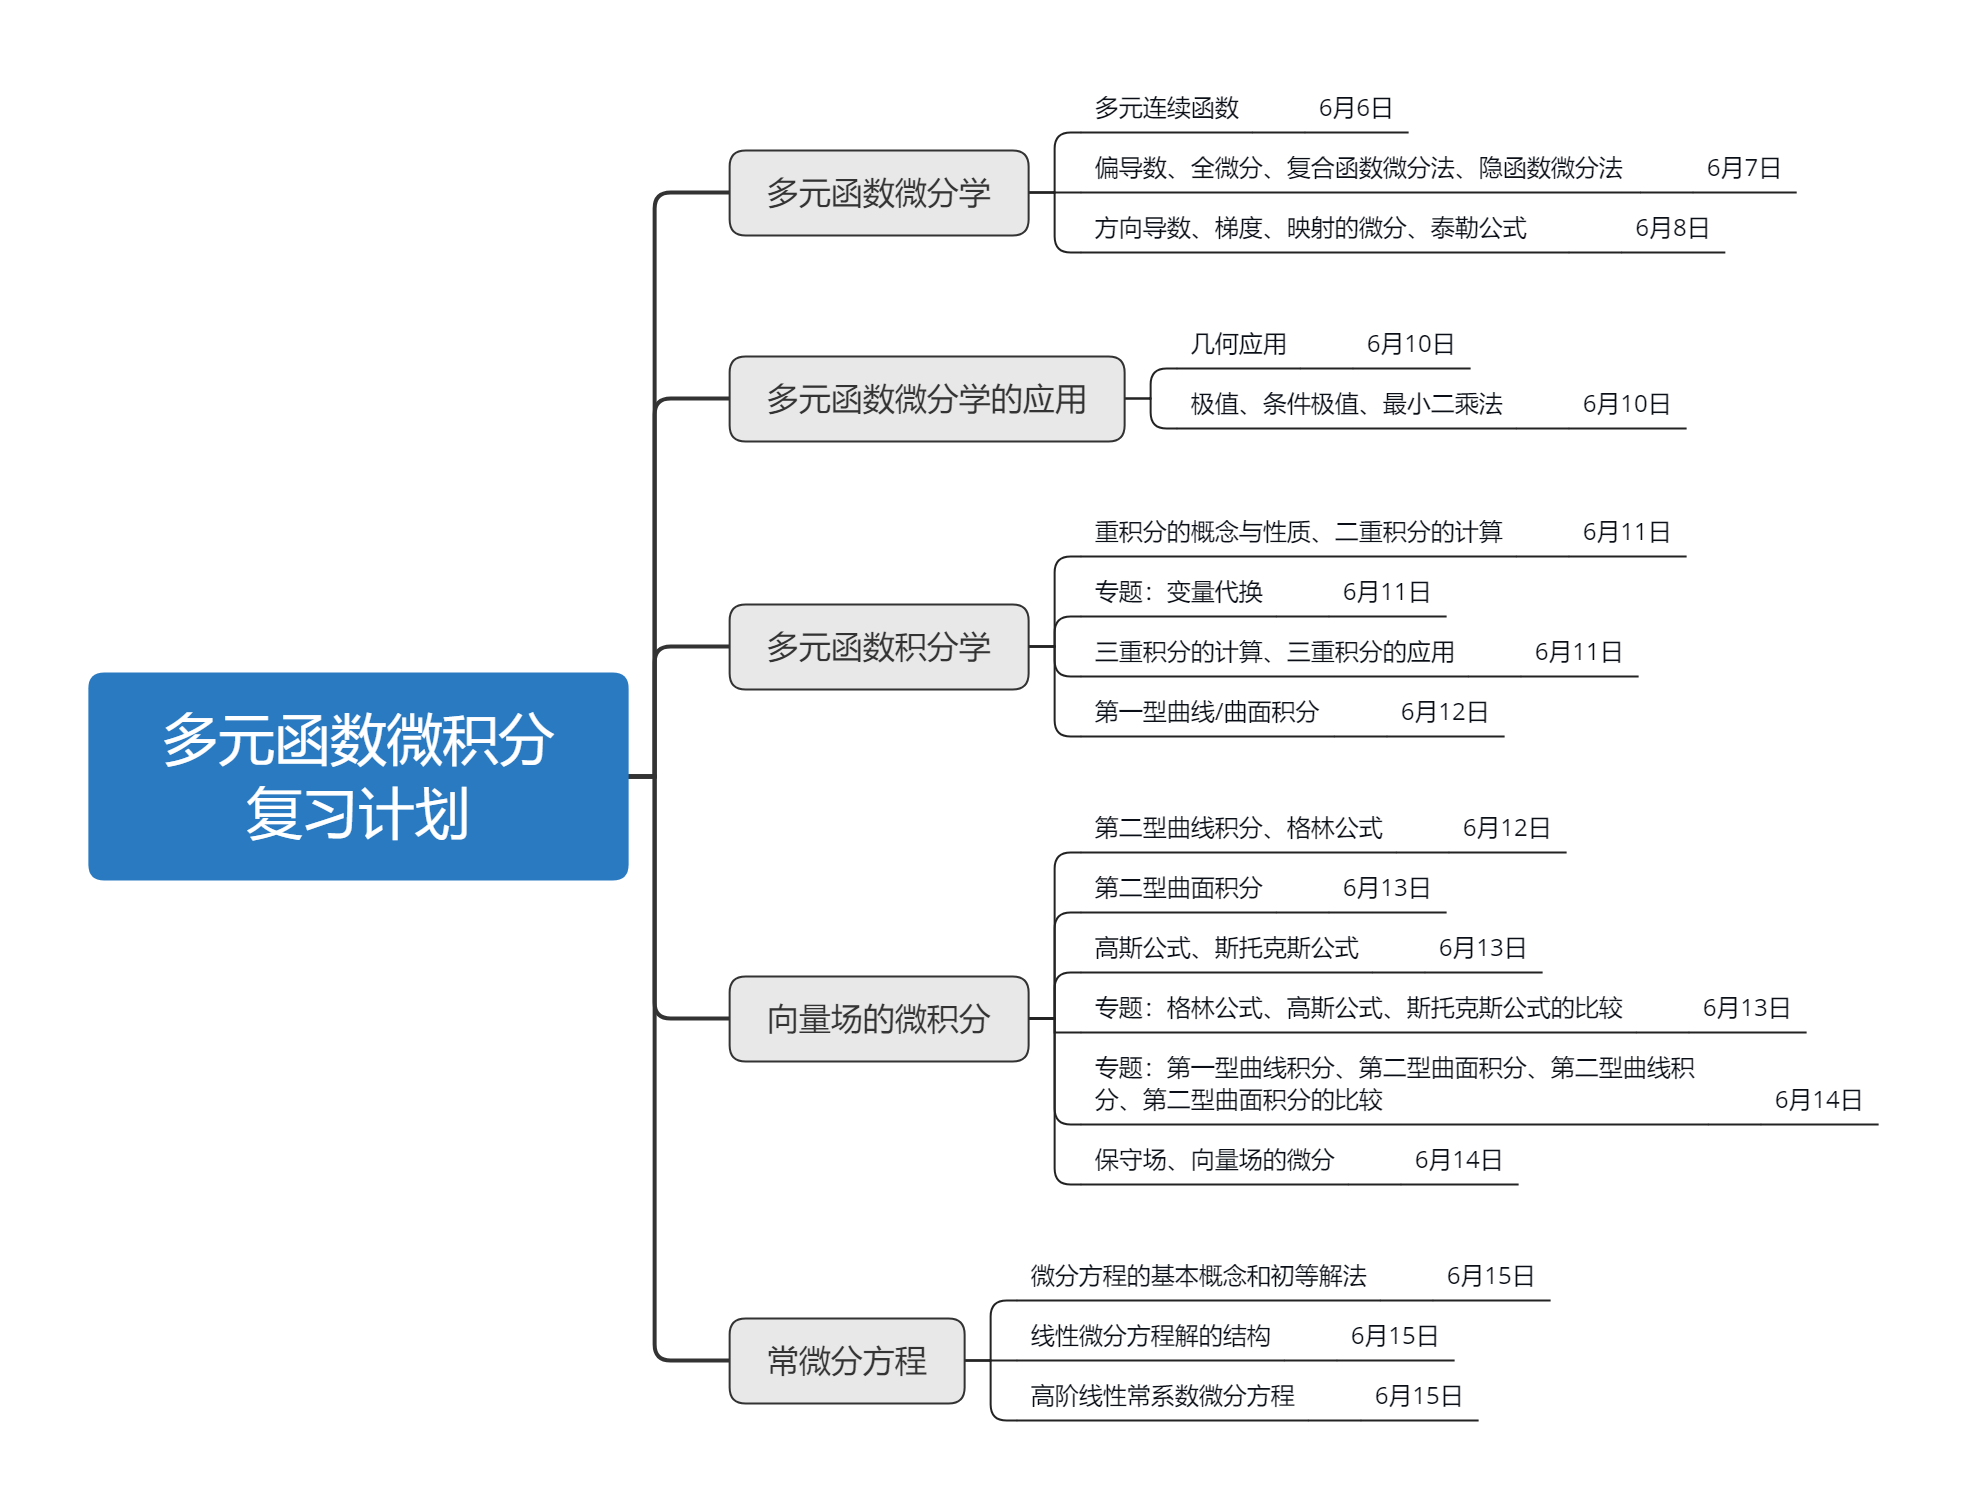
\includegraphics[height=0.5\textheight]{Figures20190605/plan.png}
\end{center}
\end{figure}
\item 复习的目标:帮助大家搭建知识结构,掌握基本的解题方法,打好基础.
\item 微积分是极重要的数学基础课,希望大家尽可能打好基础.
\item 我负责基础内容的复习,对于一些进阶的内容,大家可以复习其他习题课或讨论课上的题目,或者以前的考题,也可以自己找一些习题集.
\item 多做题、多训练对数学的掌握很重要,一些解题思路和方法,自己做题多了,训练得多了自然就容易想到了,所以鼓励大家多做题,除了书上的题目之外,可以找一些课外的题目来做.
\item 复习的主要内容包括:
\begin{enumerate}
\item知识结构. 希望大家可以掌握多元函数微积分的体系结构.
\item重难点知识的解析.
\item课后习题分类和解题思路. 主要是一些基本的方法.
\item课后习题解答.
\end{enumerate}
\item 有问题可随时与我联系:赵东阳,电话、微信: 18811708556,\\
E-mail: dy-zhao14@mails.tsinghua.edu.cn
\end{itemize}
\subsection{知识结构}
\begin{figure}[H]
\begin{center}
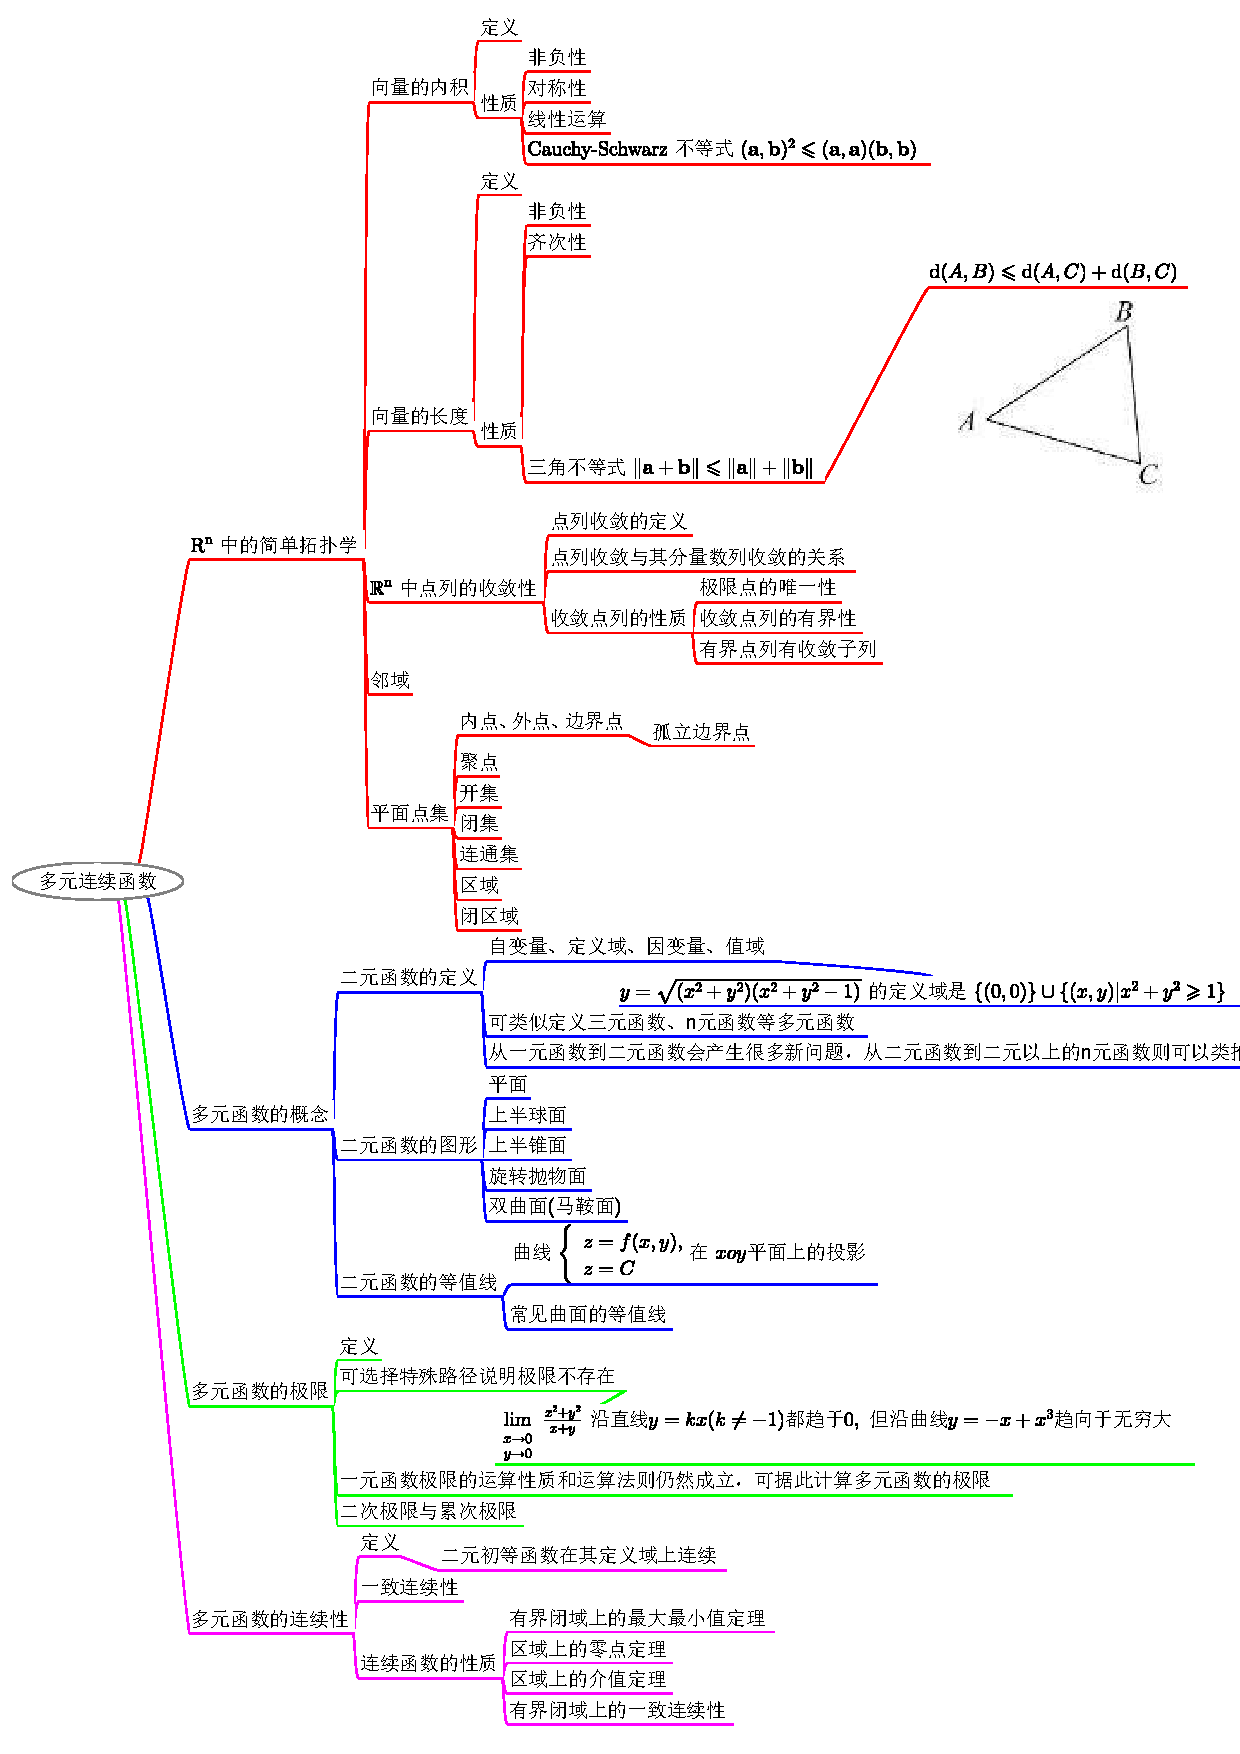
\includegraphics[height=0.95\textheight]{20190605.pdf}
\end{center}
\end{figure}
\subsection{重要图示}
\begin{enumerate}
\item平面点集
\begin{enumerate}
\item[(1)]内点、外点、边界点、聚点

点集$D$的聚点:对于任意给定的$\delta>0$, 点$P$的去心邻域$N^0(P,\delta)$内总有$D$中的点, 如$P_1,P_3$, 外点$P_2$和孤立边界点$P_4$为非聚点.
\begin{figure}[H]
\begin{center}
	\subfloat[内点$P_1$、外点$P_2$、边界点$P_3$]{{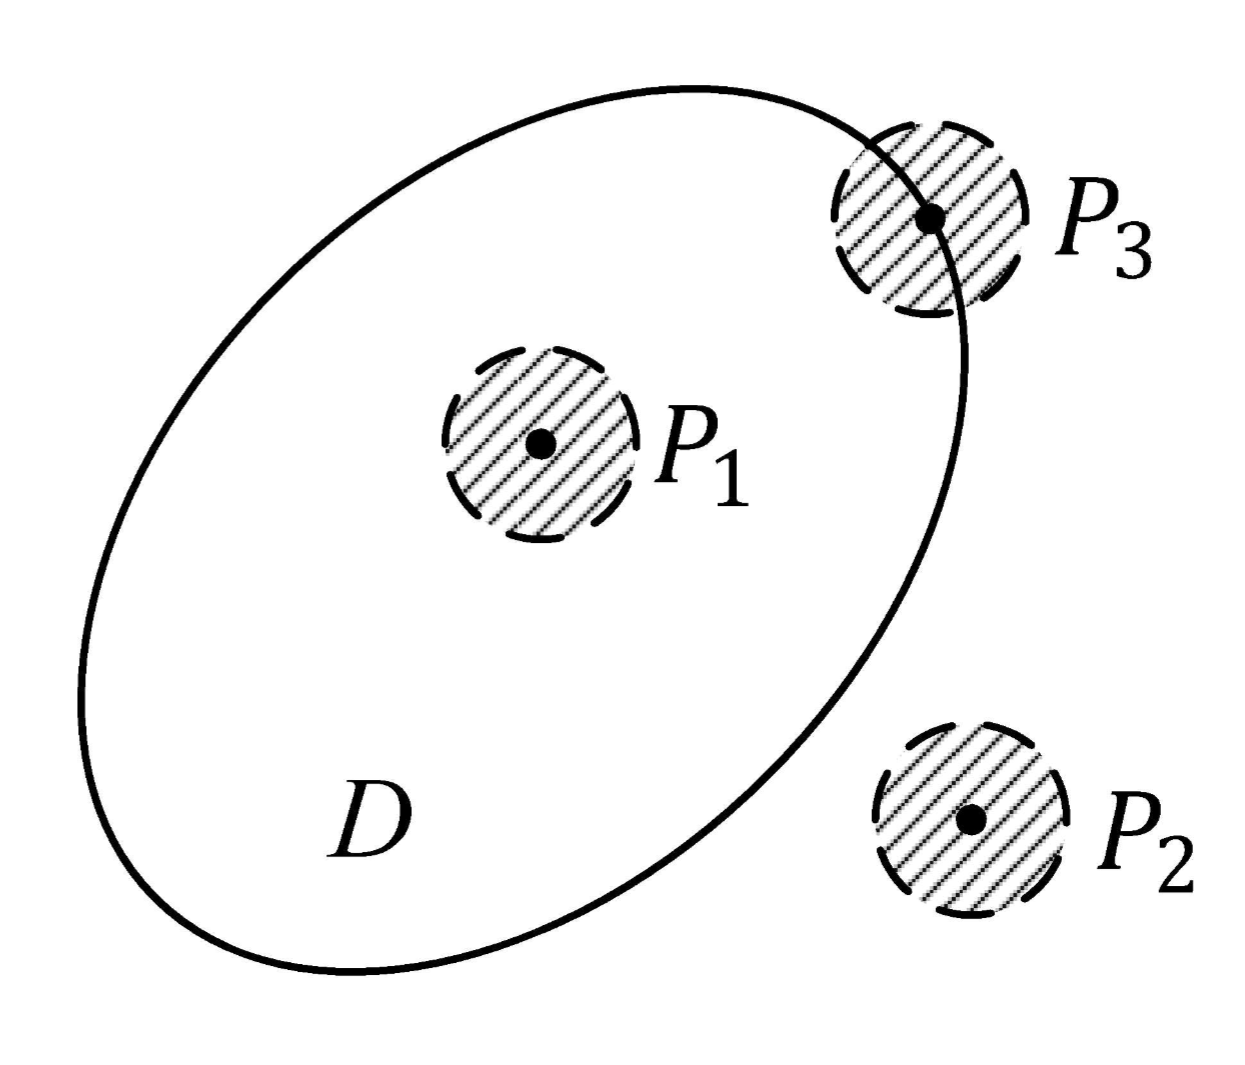
\includegraphics[height=0.3\textheight]{Figures20190605/Internal_external_boundarypoints.PNG} }}
	\subfloat[孤立边界点$P_4$]{{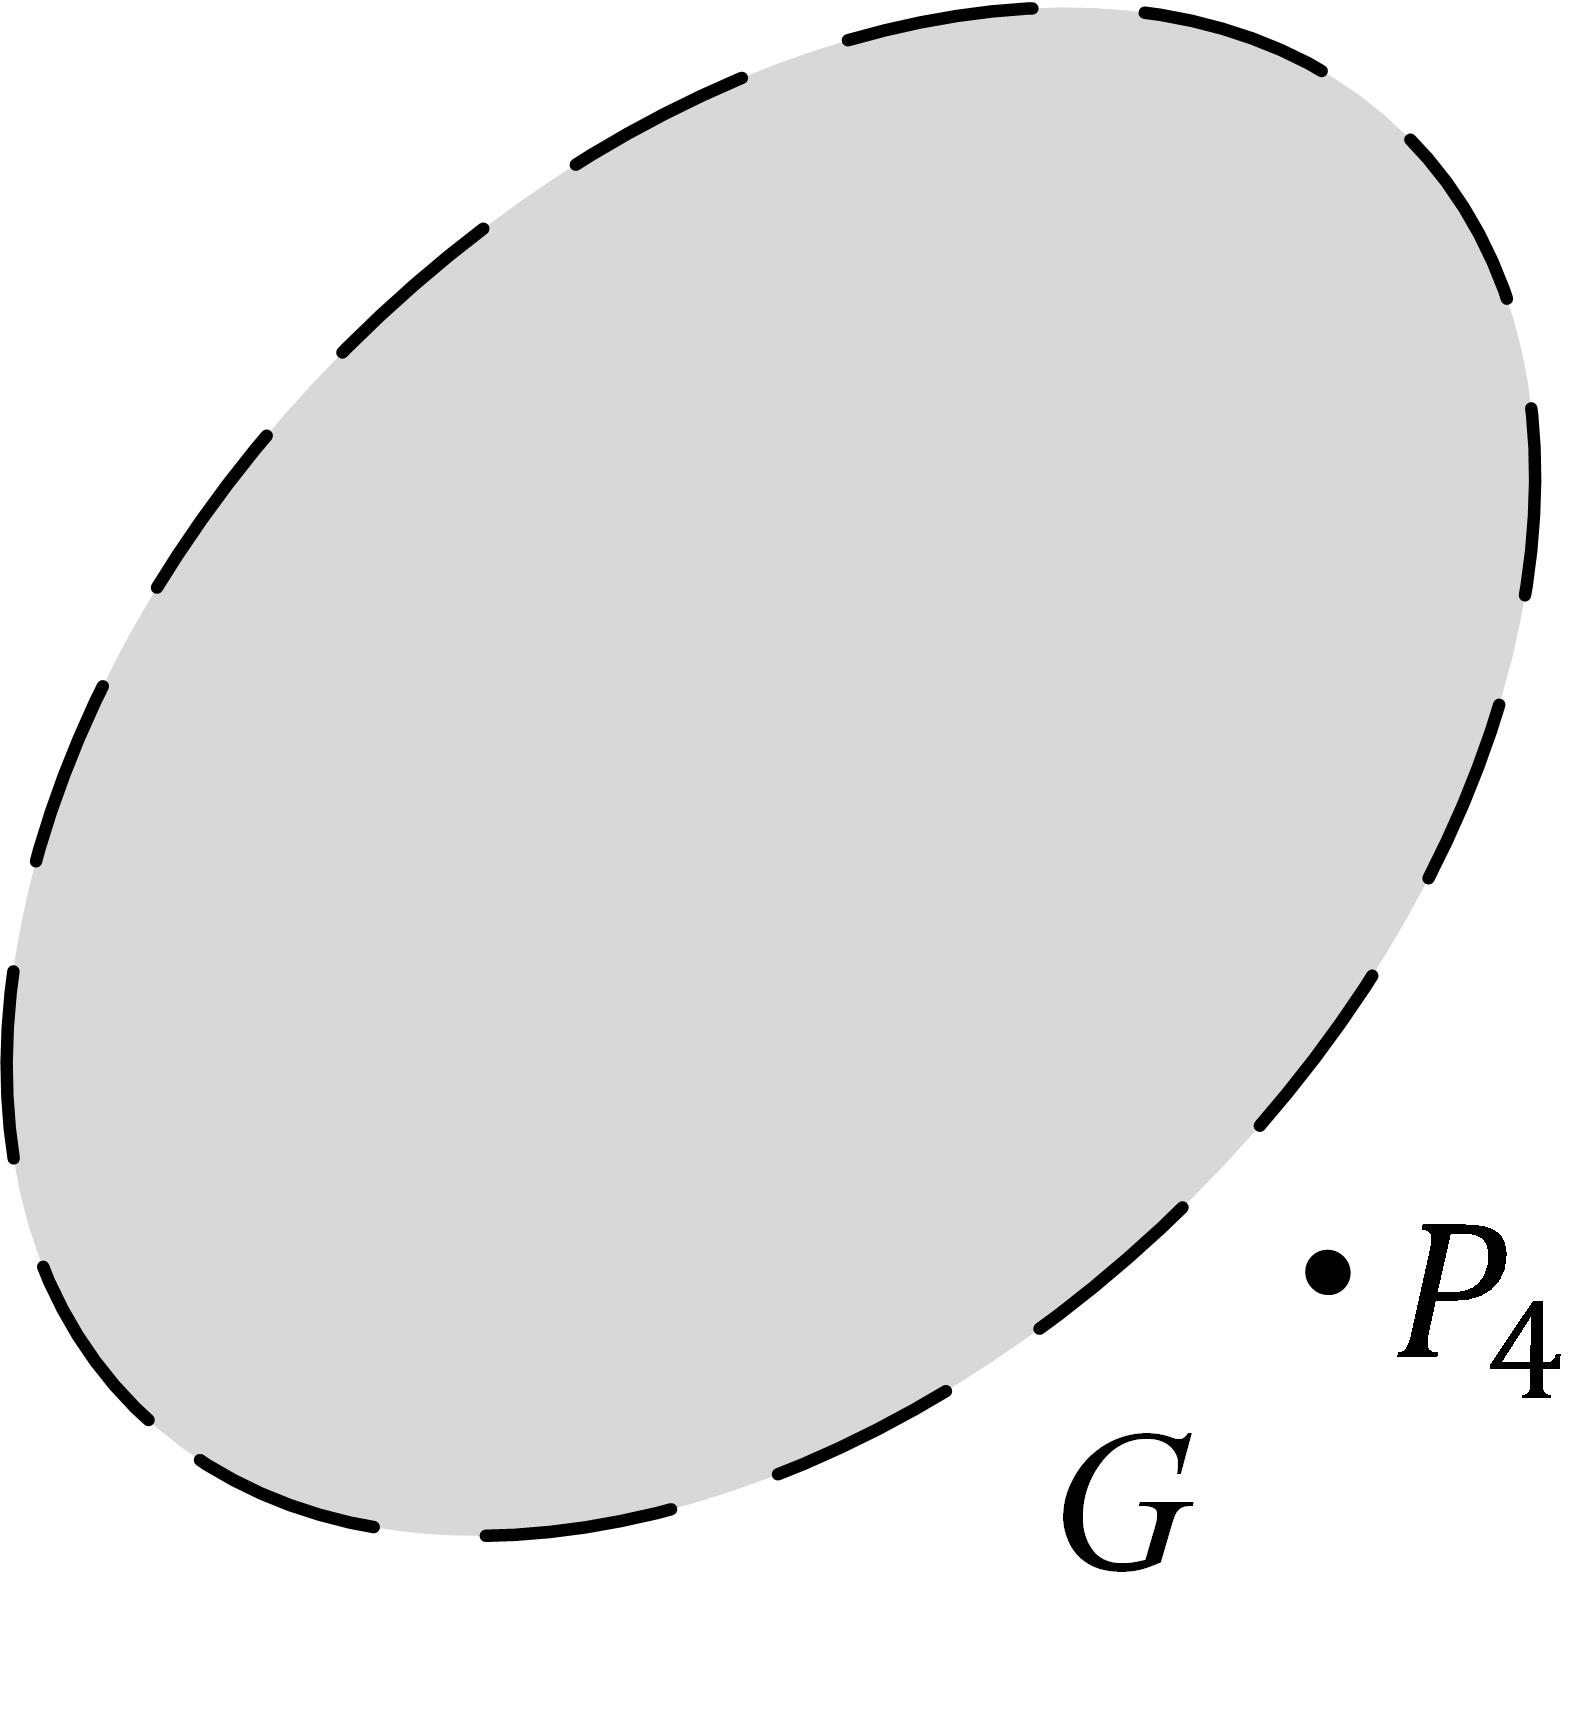
\includegraphics[height=0.3\textheight]{Figures20190605/dependent_boundary.jpg} }}
\end{center}
\caption{内点、外点、边界点、聚点}
\end{figure}
\item[(2)]开集、闭集、连通集、非连通集
\begin{figure}[H]
\begin{center}
	\subfloat[开集(内点的集合)]{{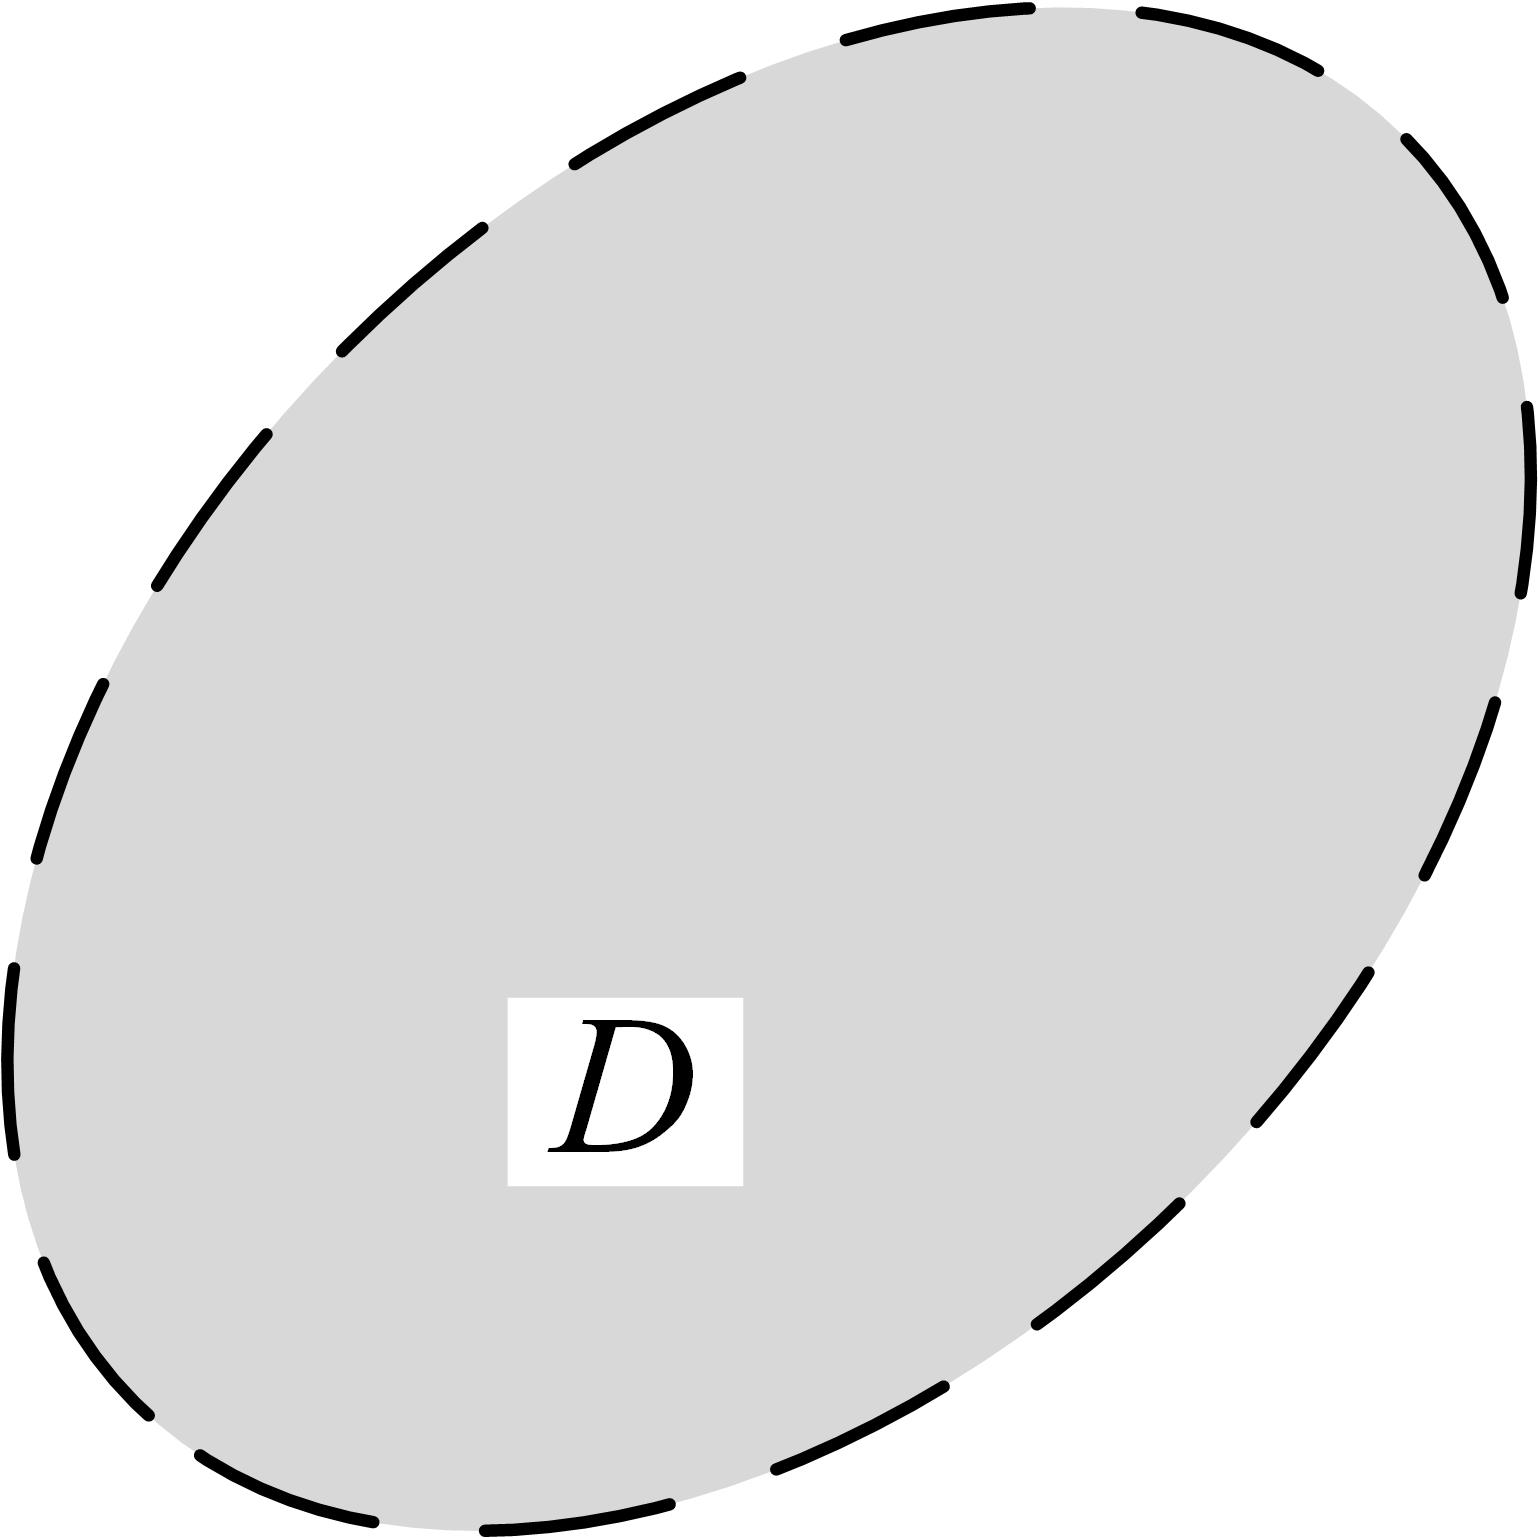
\includegraphics[height=0.15\textheight]{Figures20190605/openset.jpg} }}
	\subfloat[闭集(第一象限,含原点及$x,y$轴正半轴,其补集是开集,故是闭集)]{{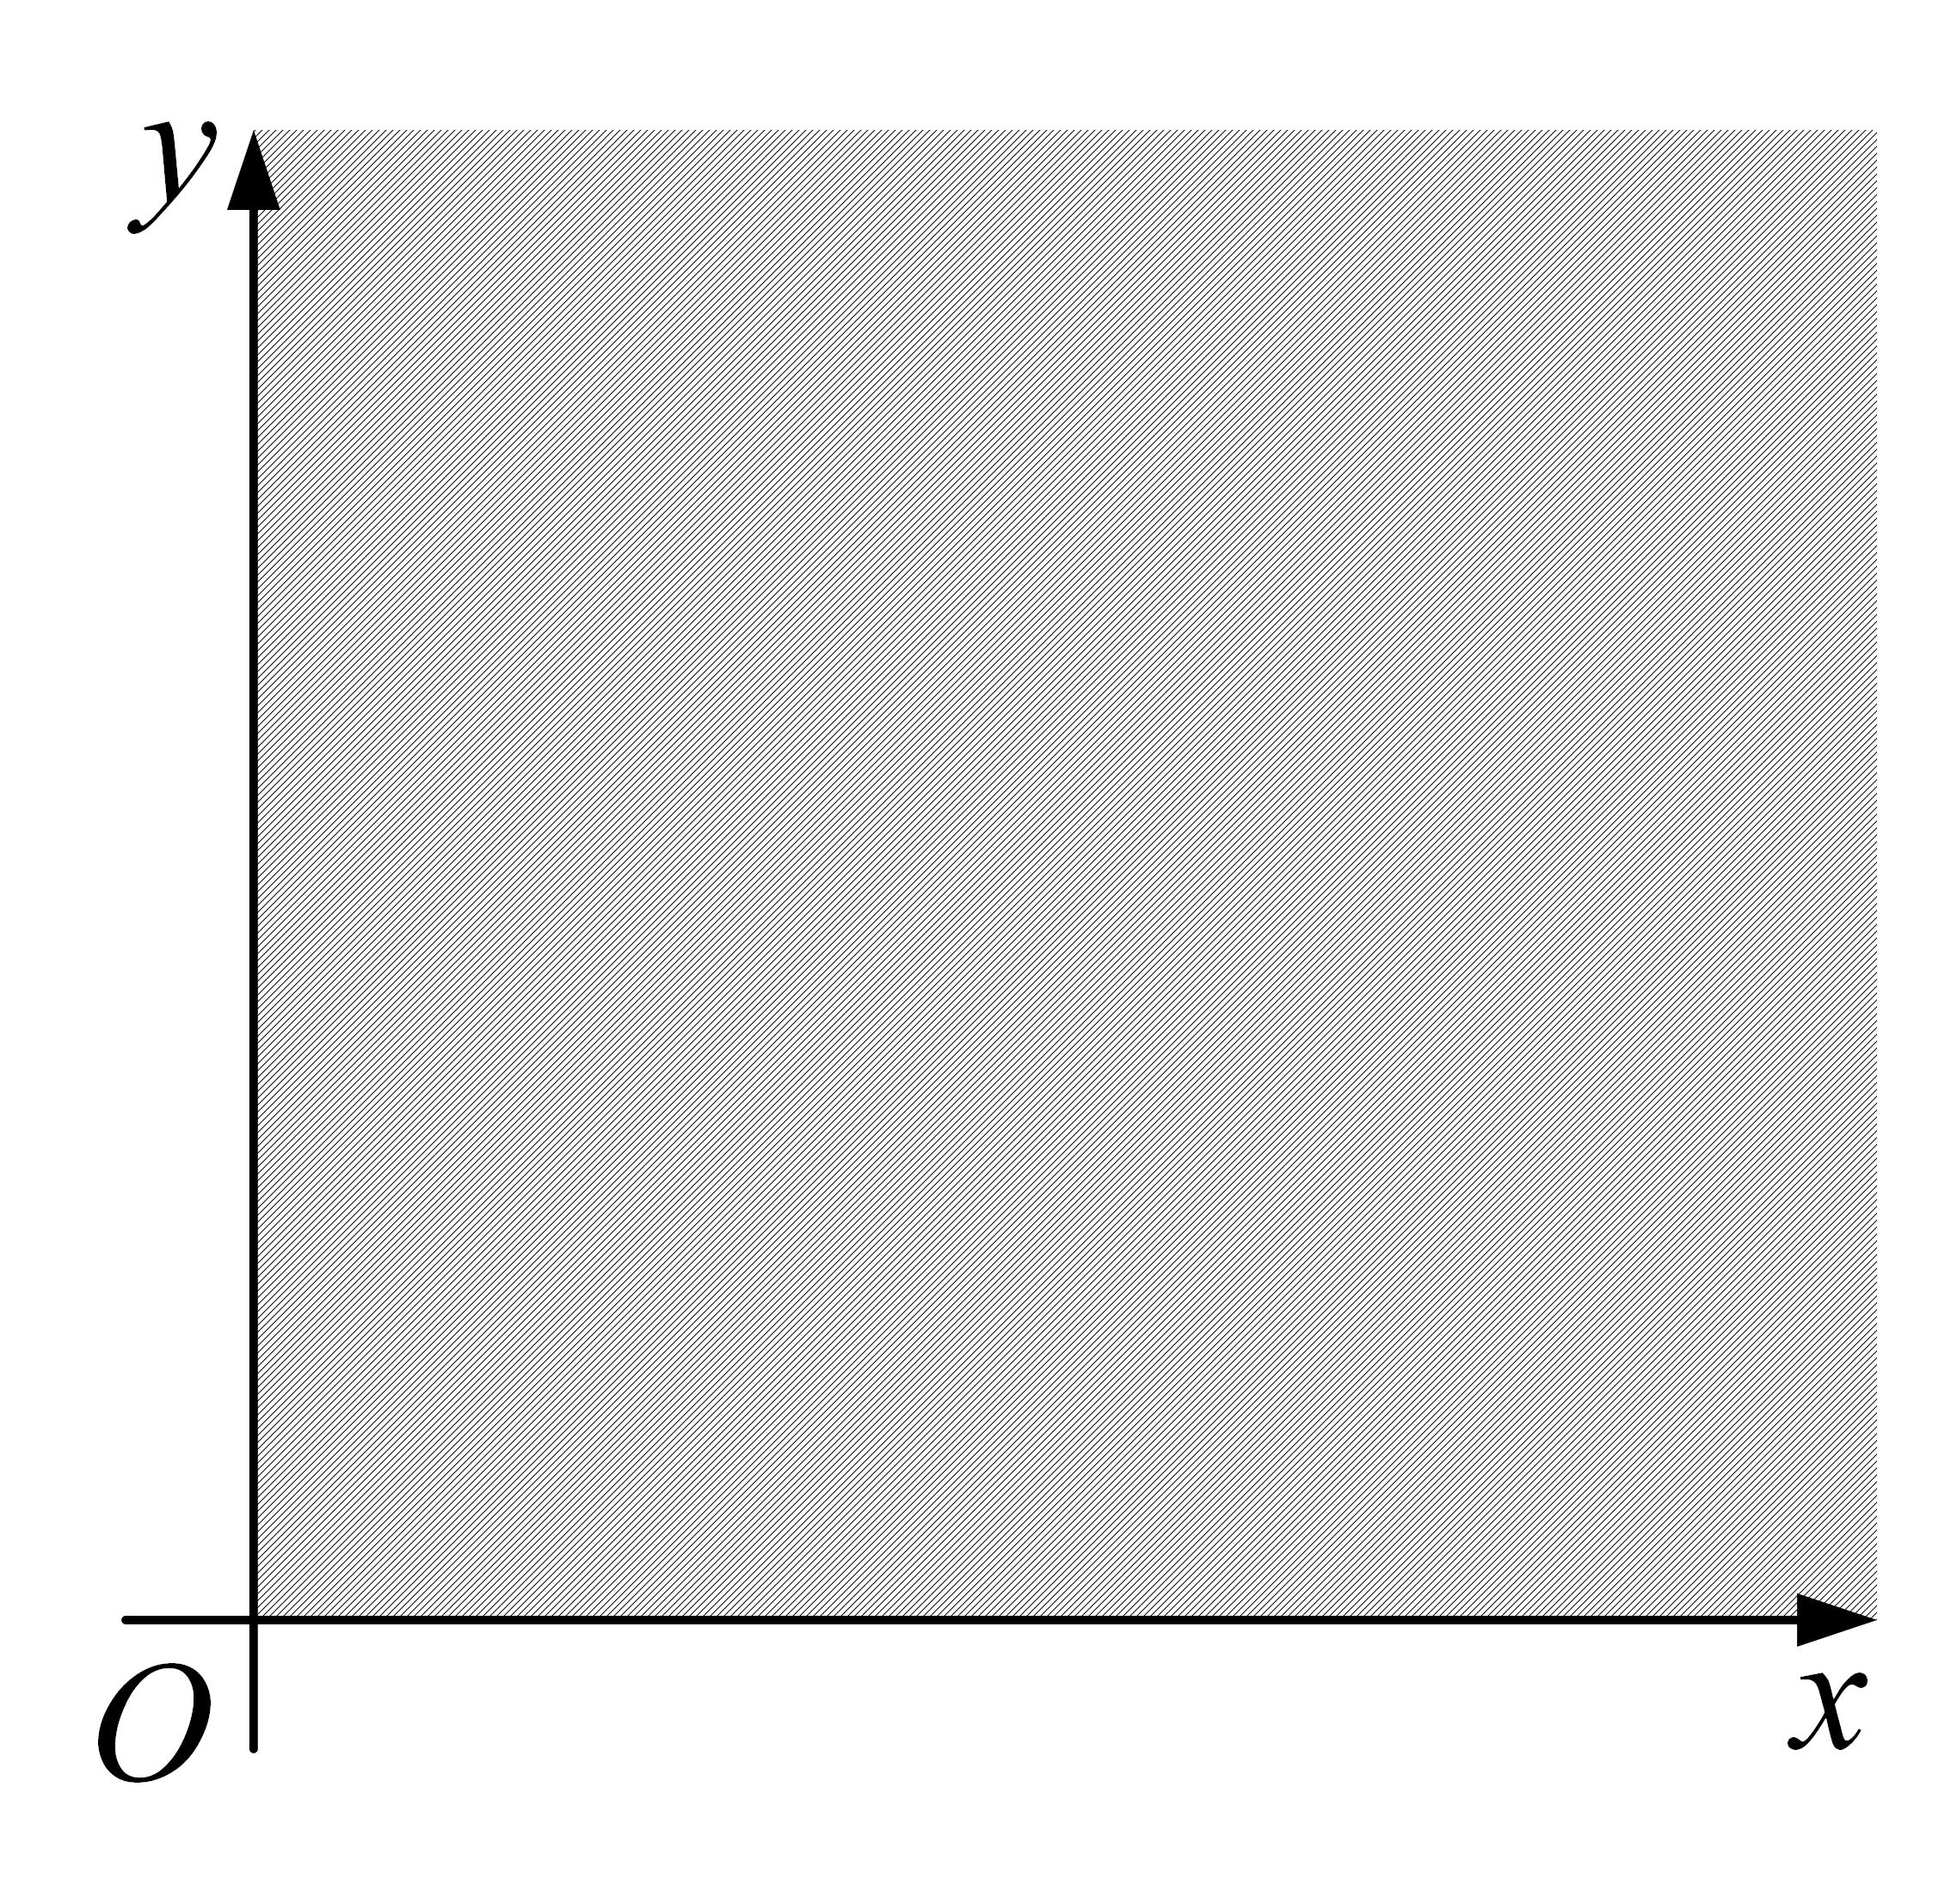
\includegraphics[height=0.15\textheight]{Figures20190605/closedset.jpg} }}
	\subfloat[连通集]{{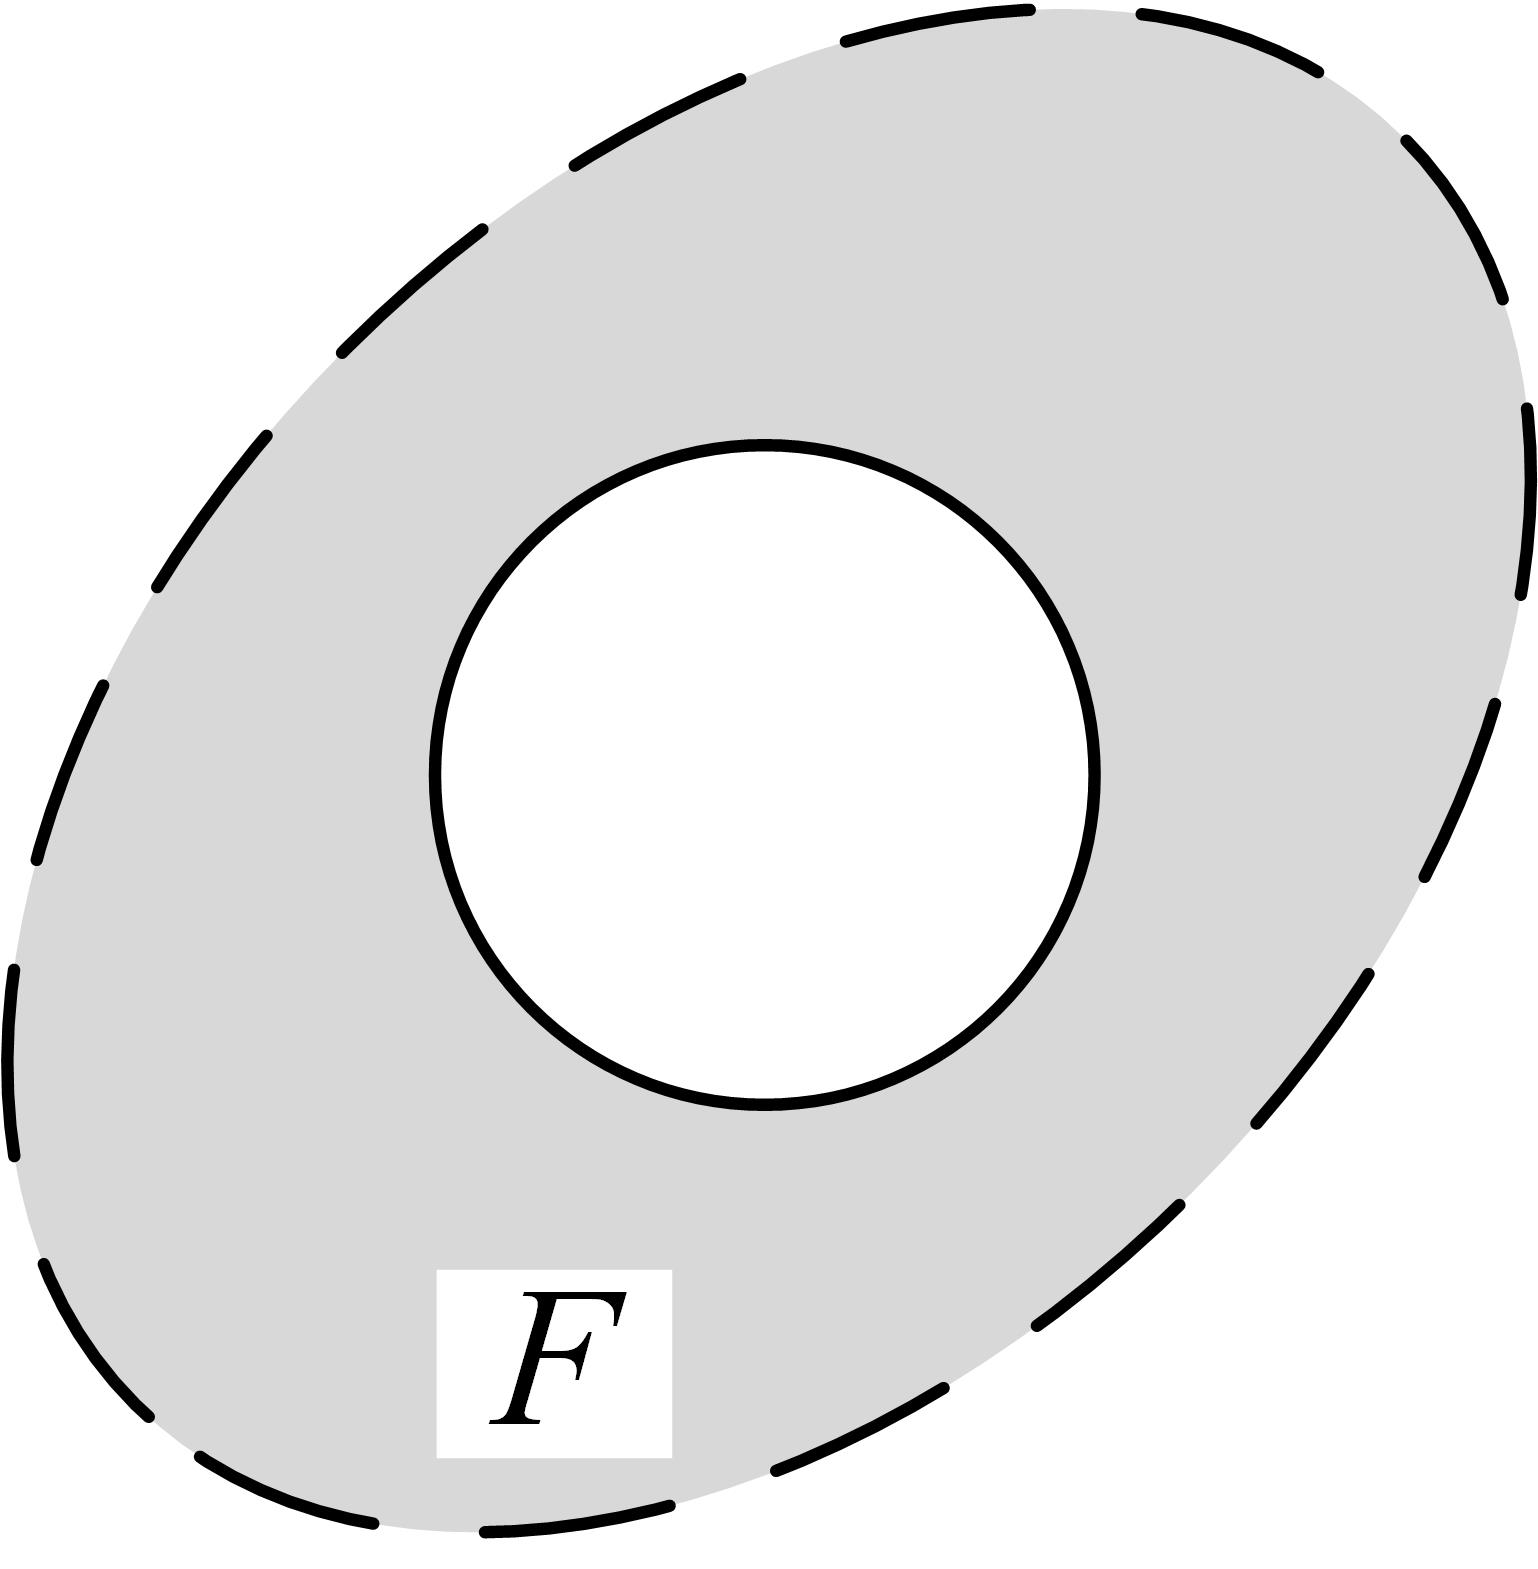
\includegraphics[height=0.15\textheight]{Figures20190605/connectedset.jpg} }}
	\subfloat[非连通集]{{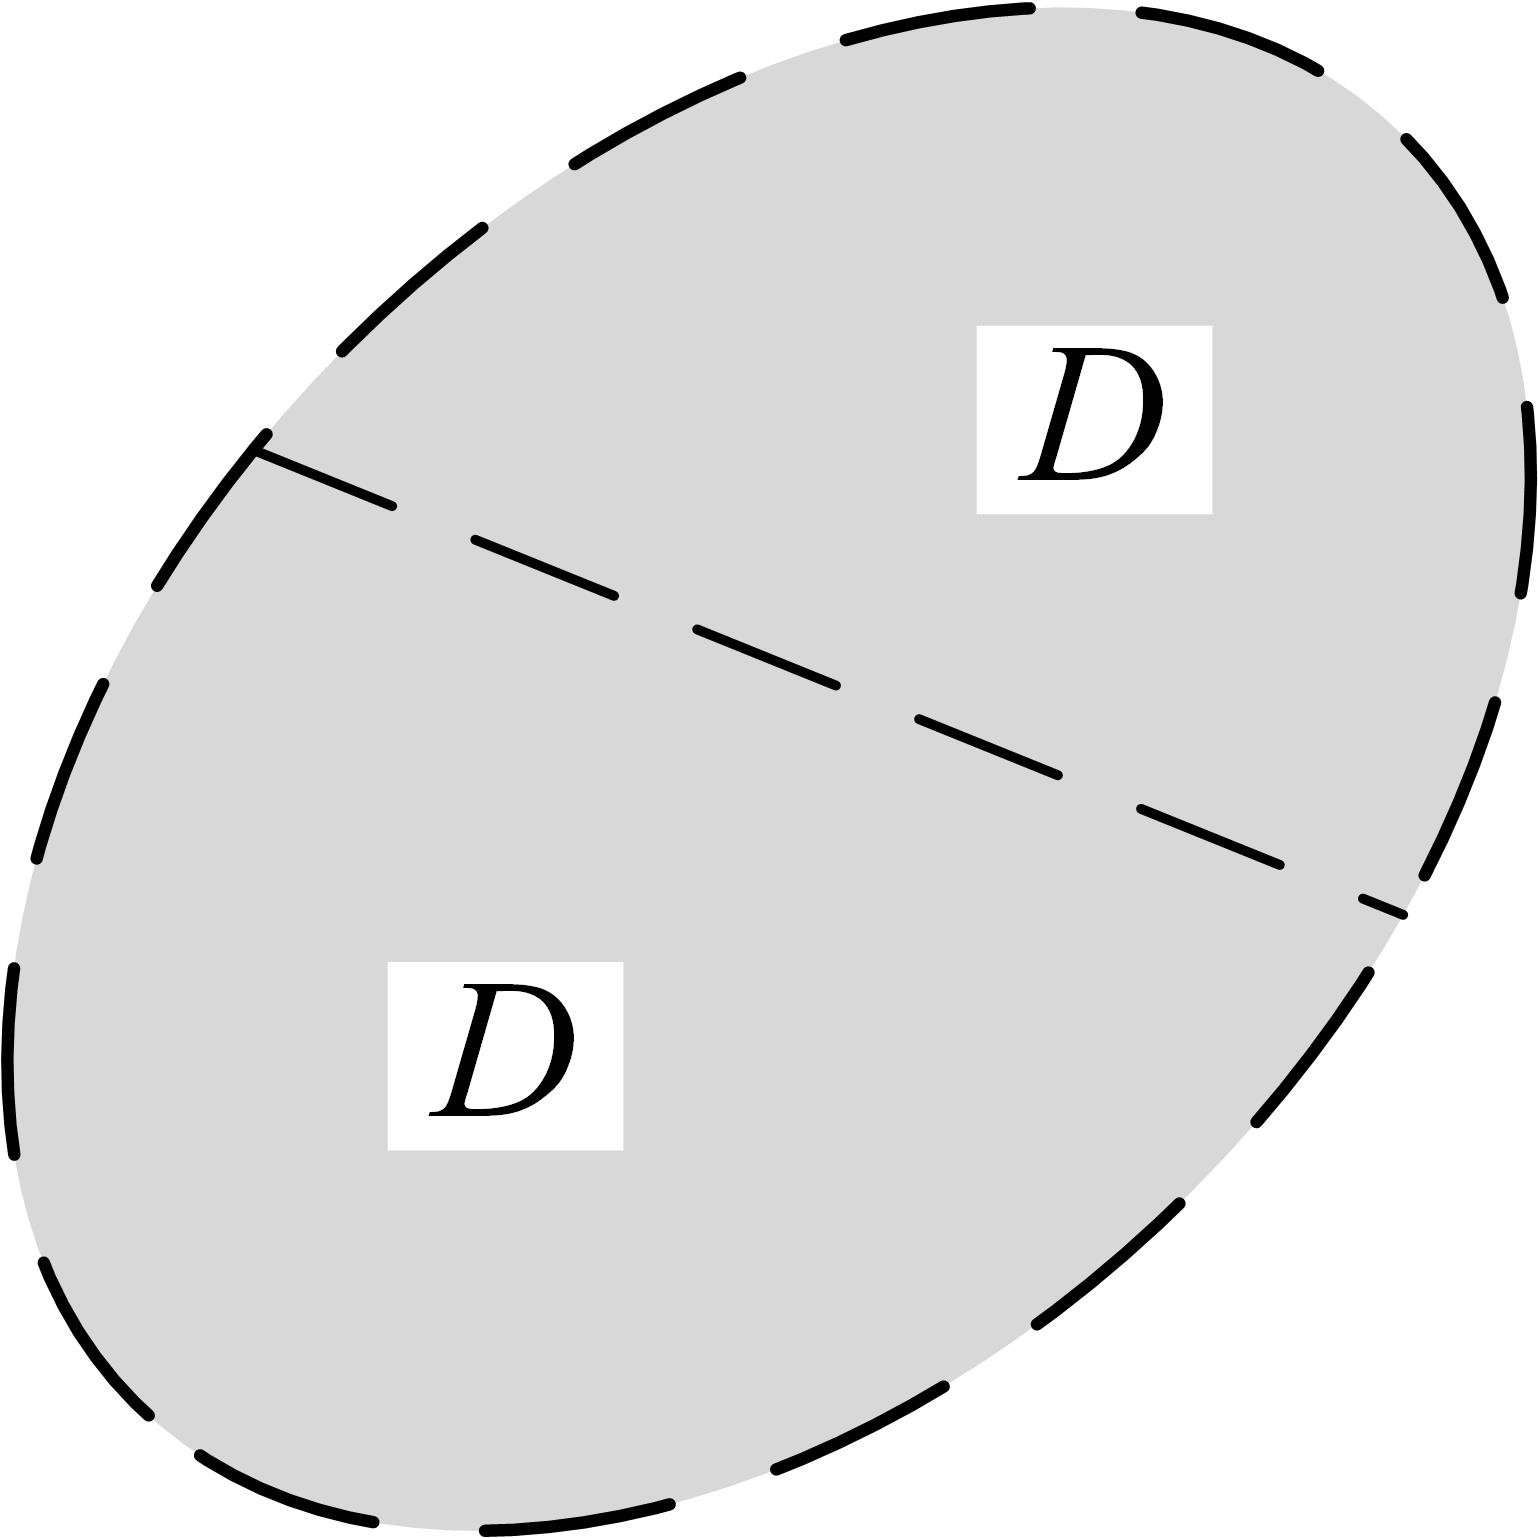
\includegraphics[height=0.15\textheight]{Figures20190605/nonconnectedset.jpg} }}
\end{center}
\caption{开集、闭集、连通集、非连通集}
\end{figure}
\begin{enumerate}
\item[]
\end{enumerate}
\item[(3)]区域、闭区域
\begin{figure}[H]
\begin{center}
	\subfloat[区域(连通的开集)]{{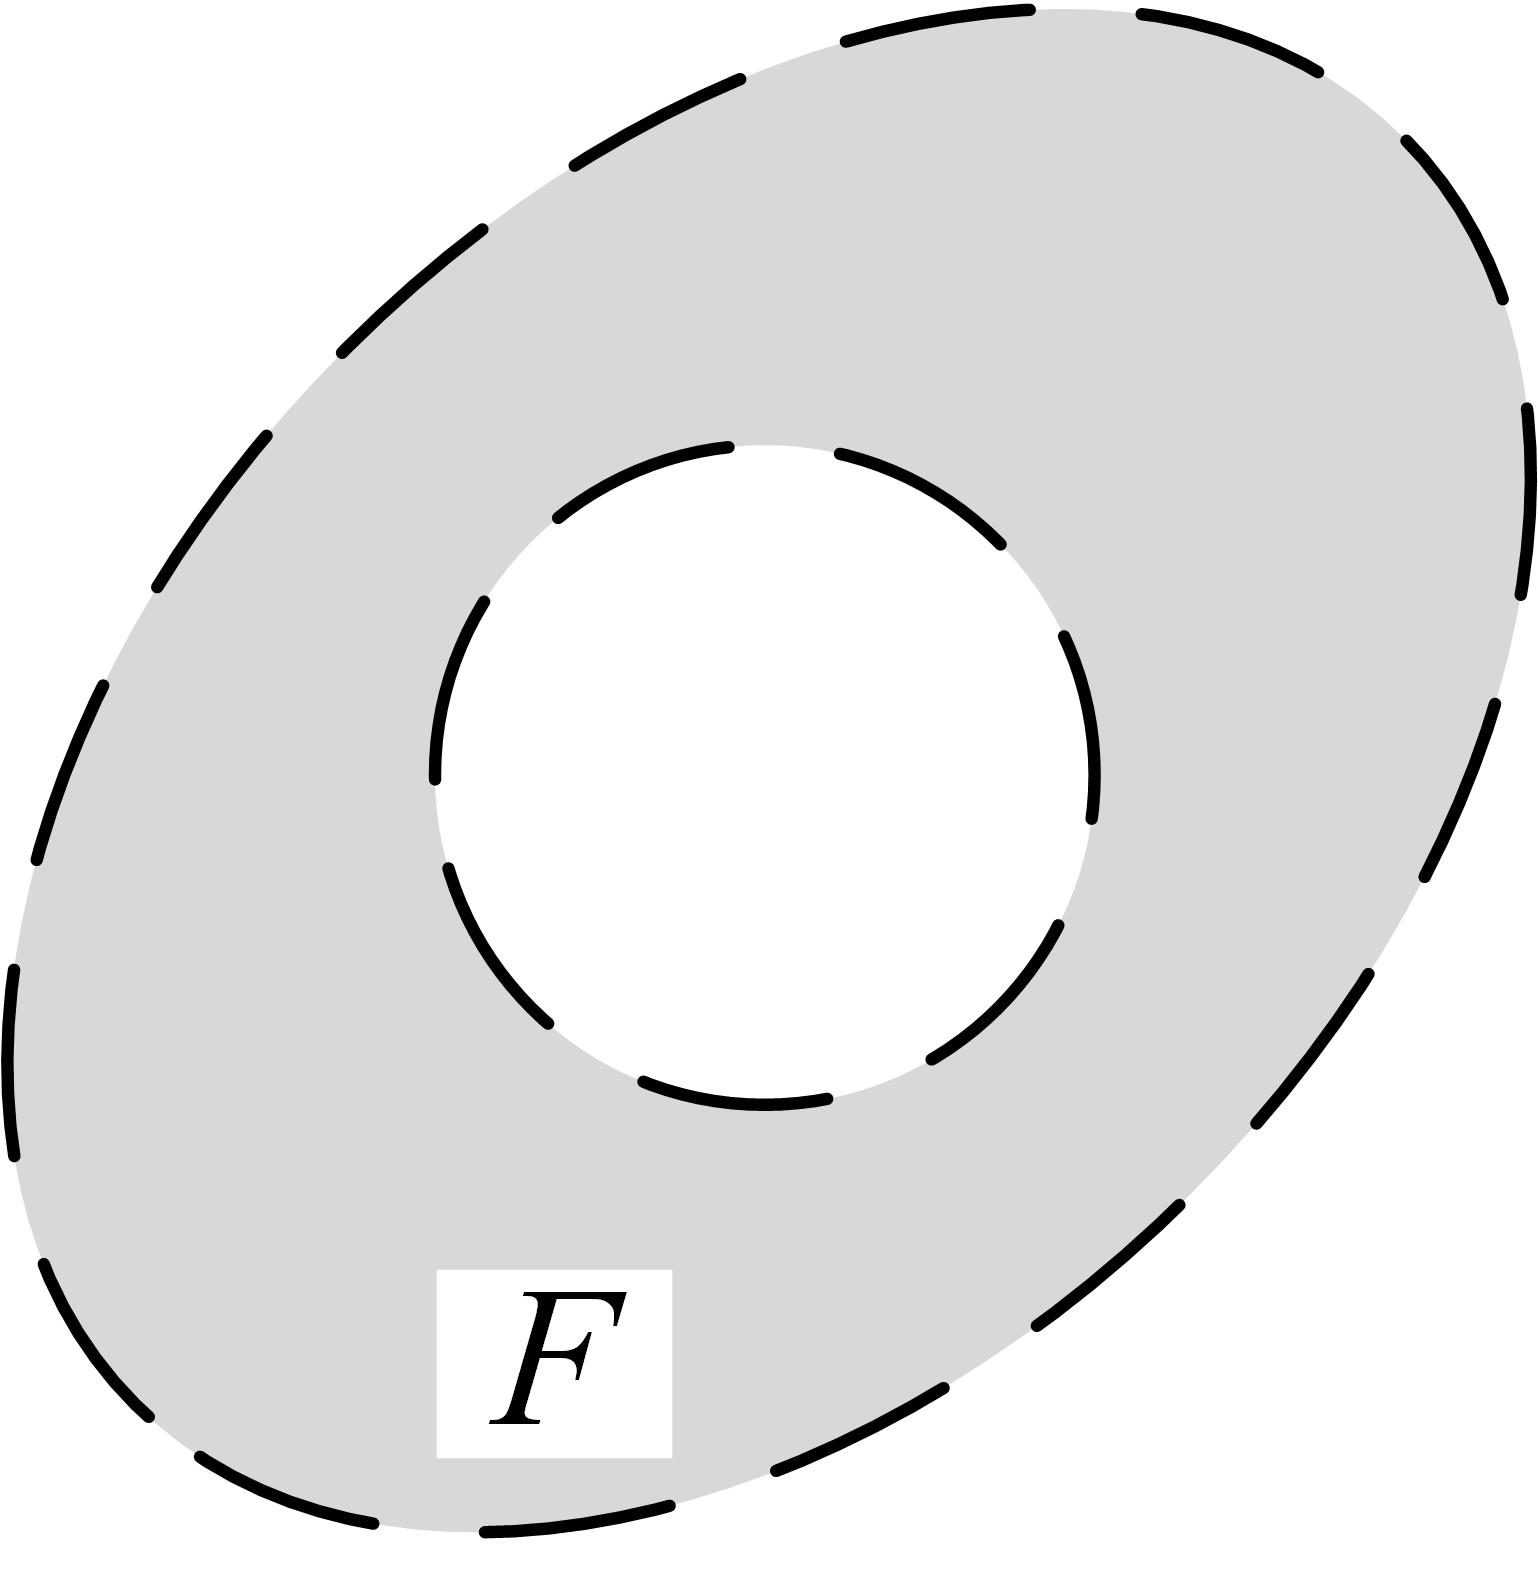
\includegraphics[height=0.3\textheight]{Figures20190605/zone.jpg} }}
	\subfloat[闭区域(区域$\cup$其边界)]{{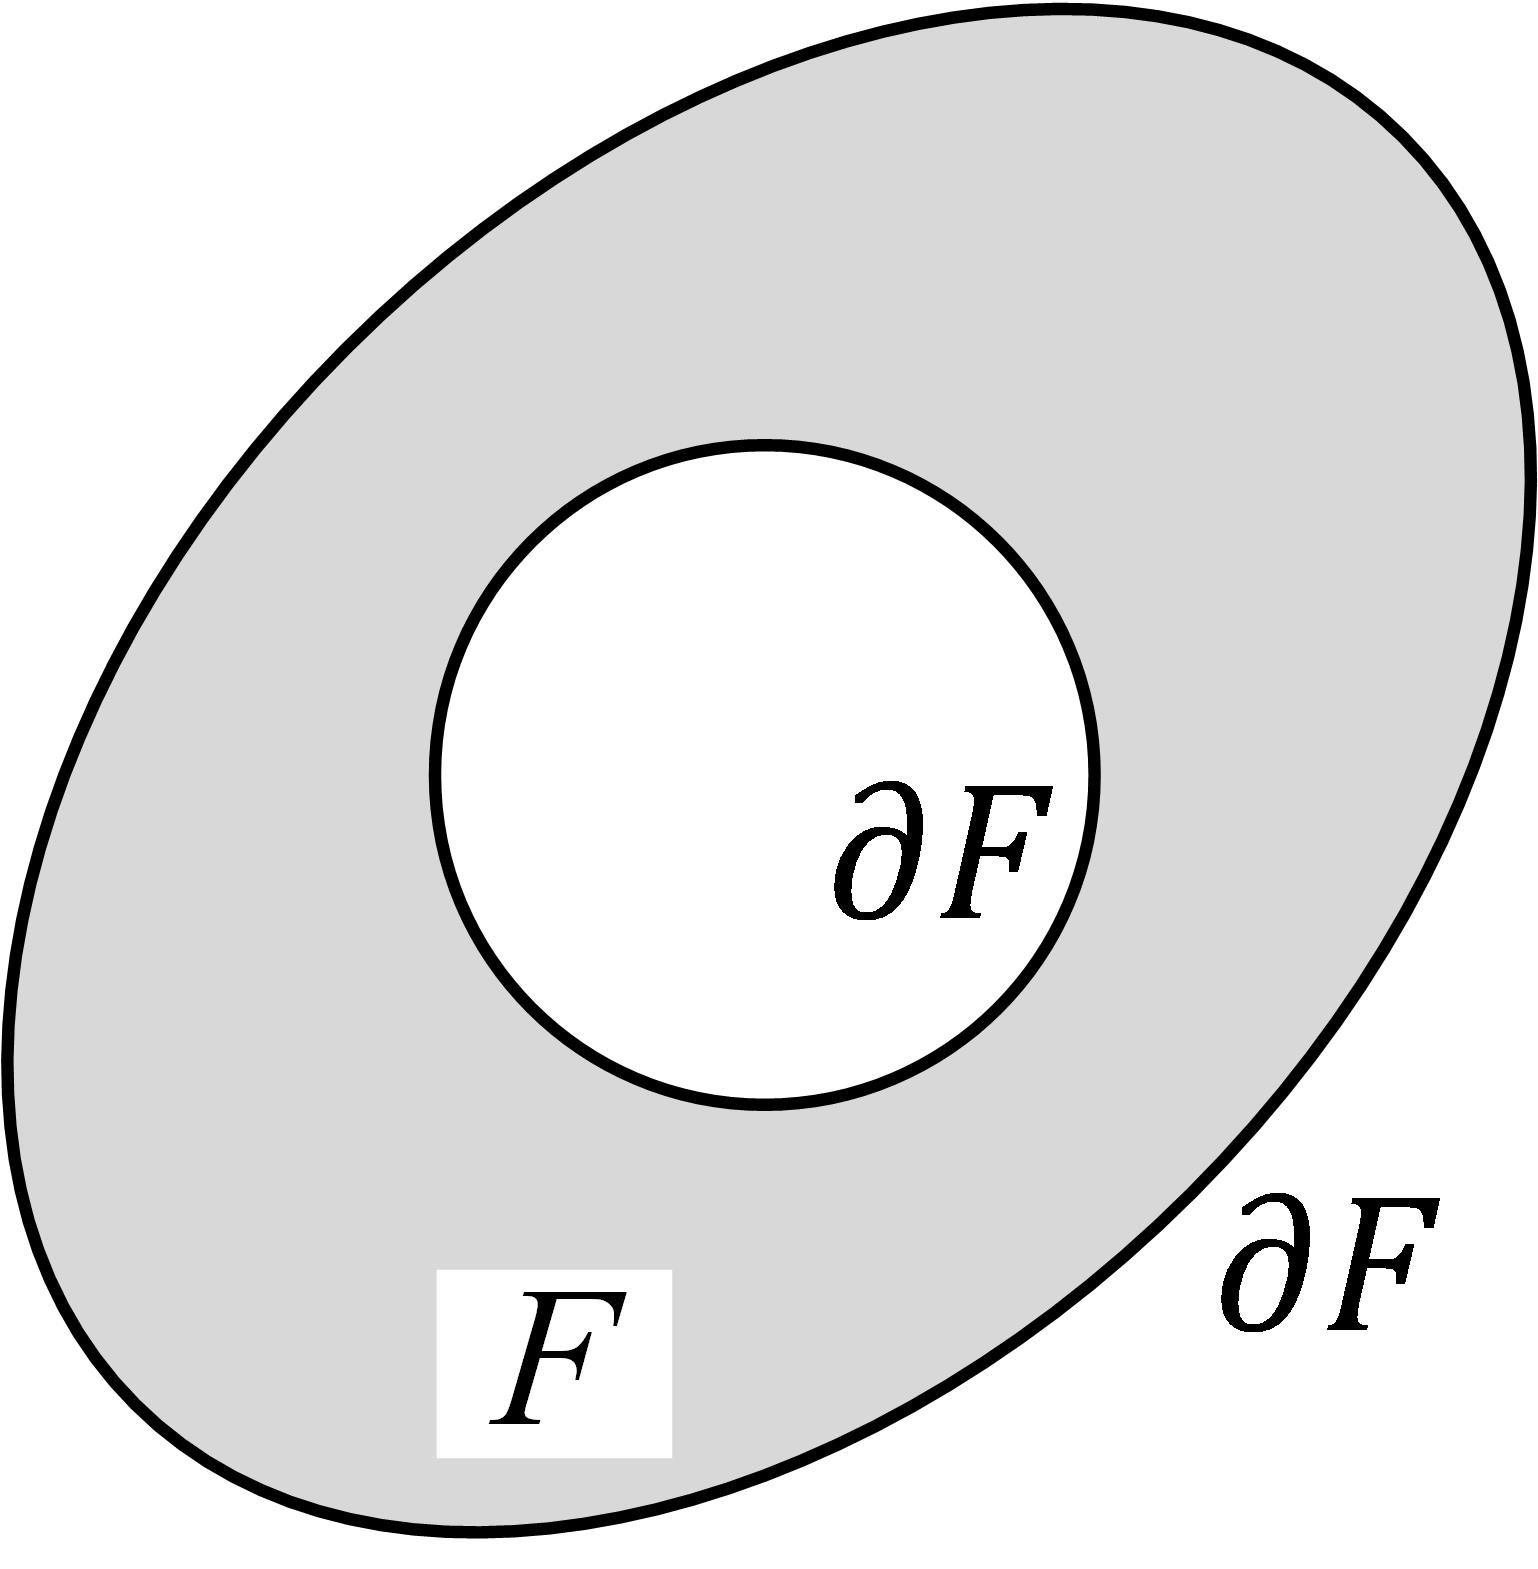
\includegraphics[height=0.3\textheight]{Figures20190605/closedzone.jpg} }}
\end{center}
\caption{区域、闭区域}
\end{figure}
\end{enumerate}
\begin{enumerate}
\item[]
\item[]
\item[]
\item[]
\item[]
\item[]
\item[]
\item[]
\item[]
\item[]
\item[]
\item[]
\item[]
\item[]
\item[]
\end{enumerate}
\item常见二元函数的图形
\begin{figure}[H]
\begin{center}
	\subfloat[平面$z=c(1-\frac xa-\frac yb)$]{{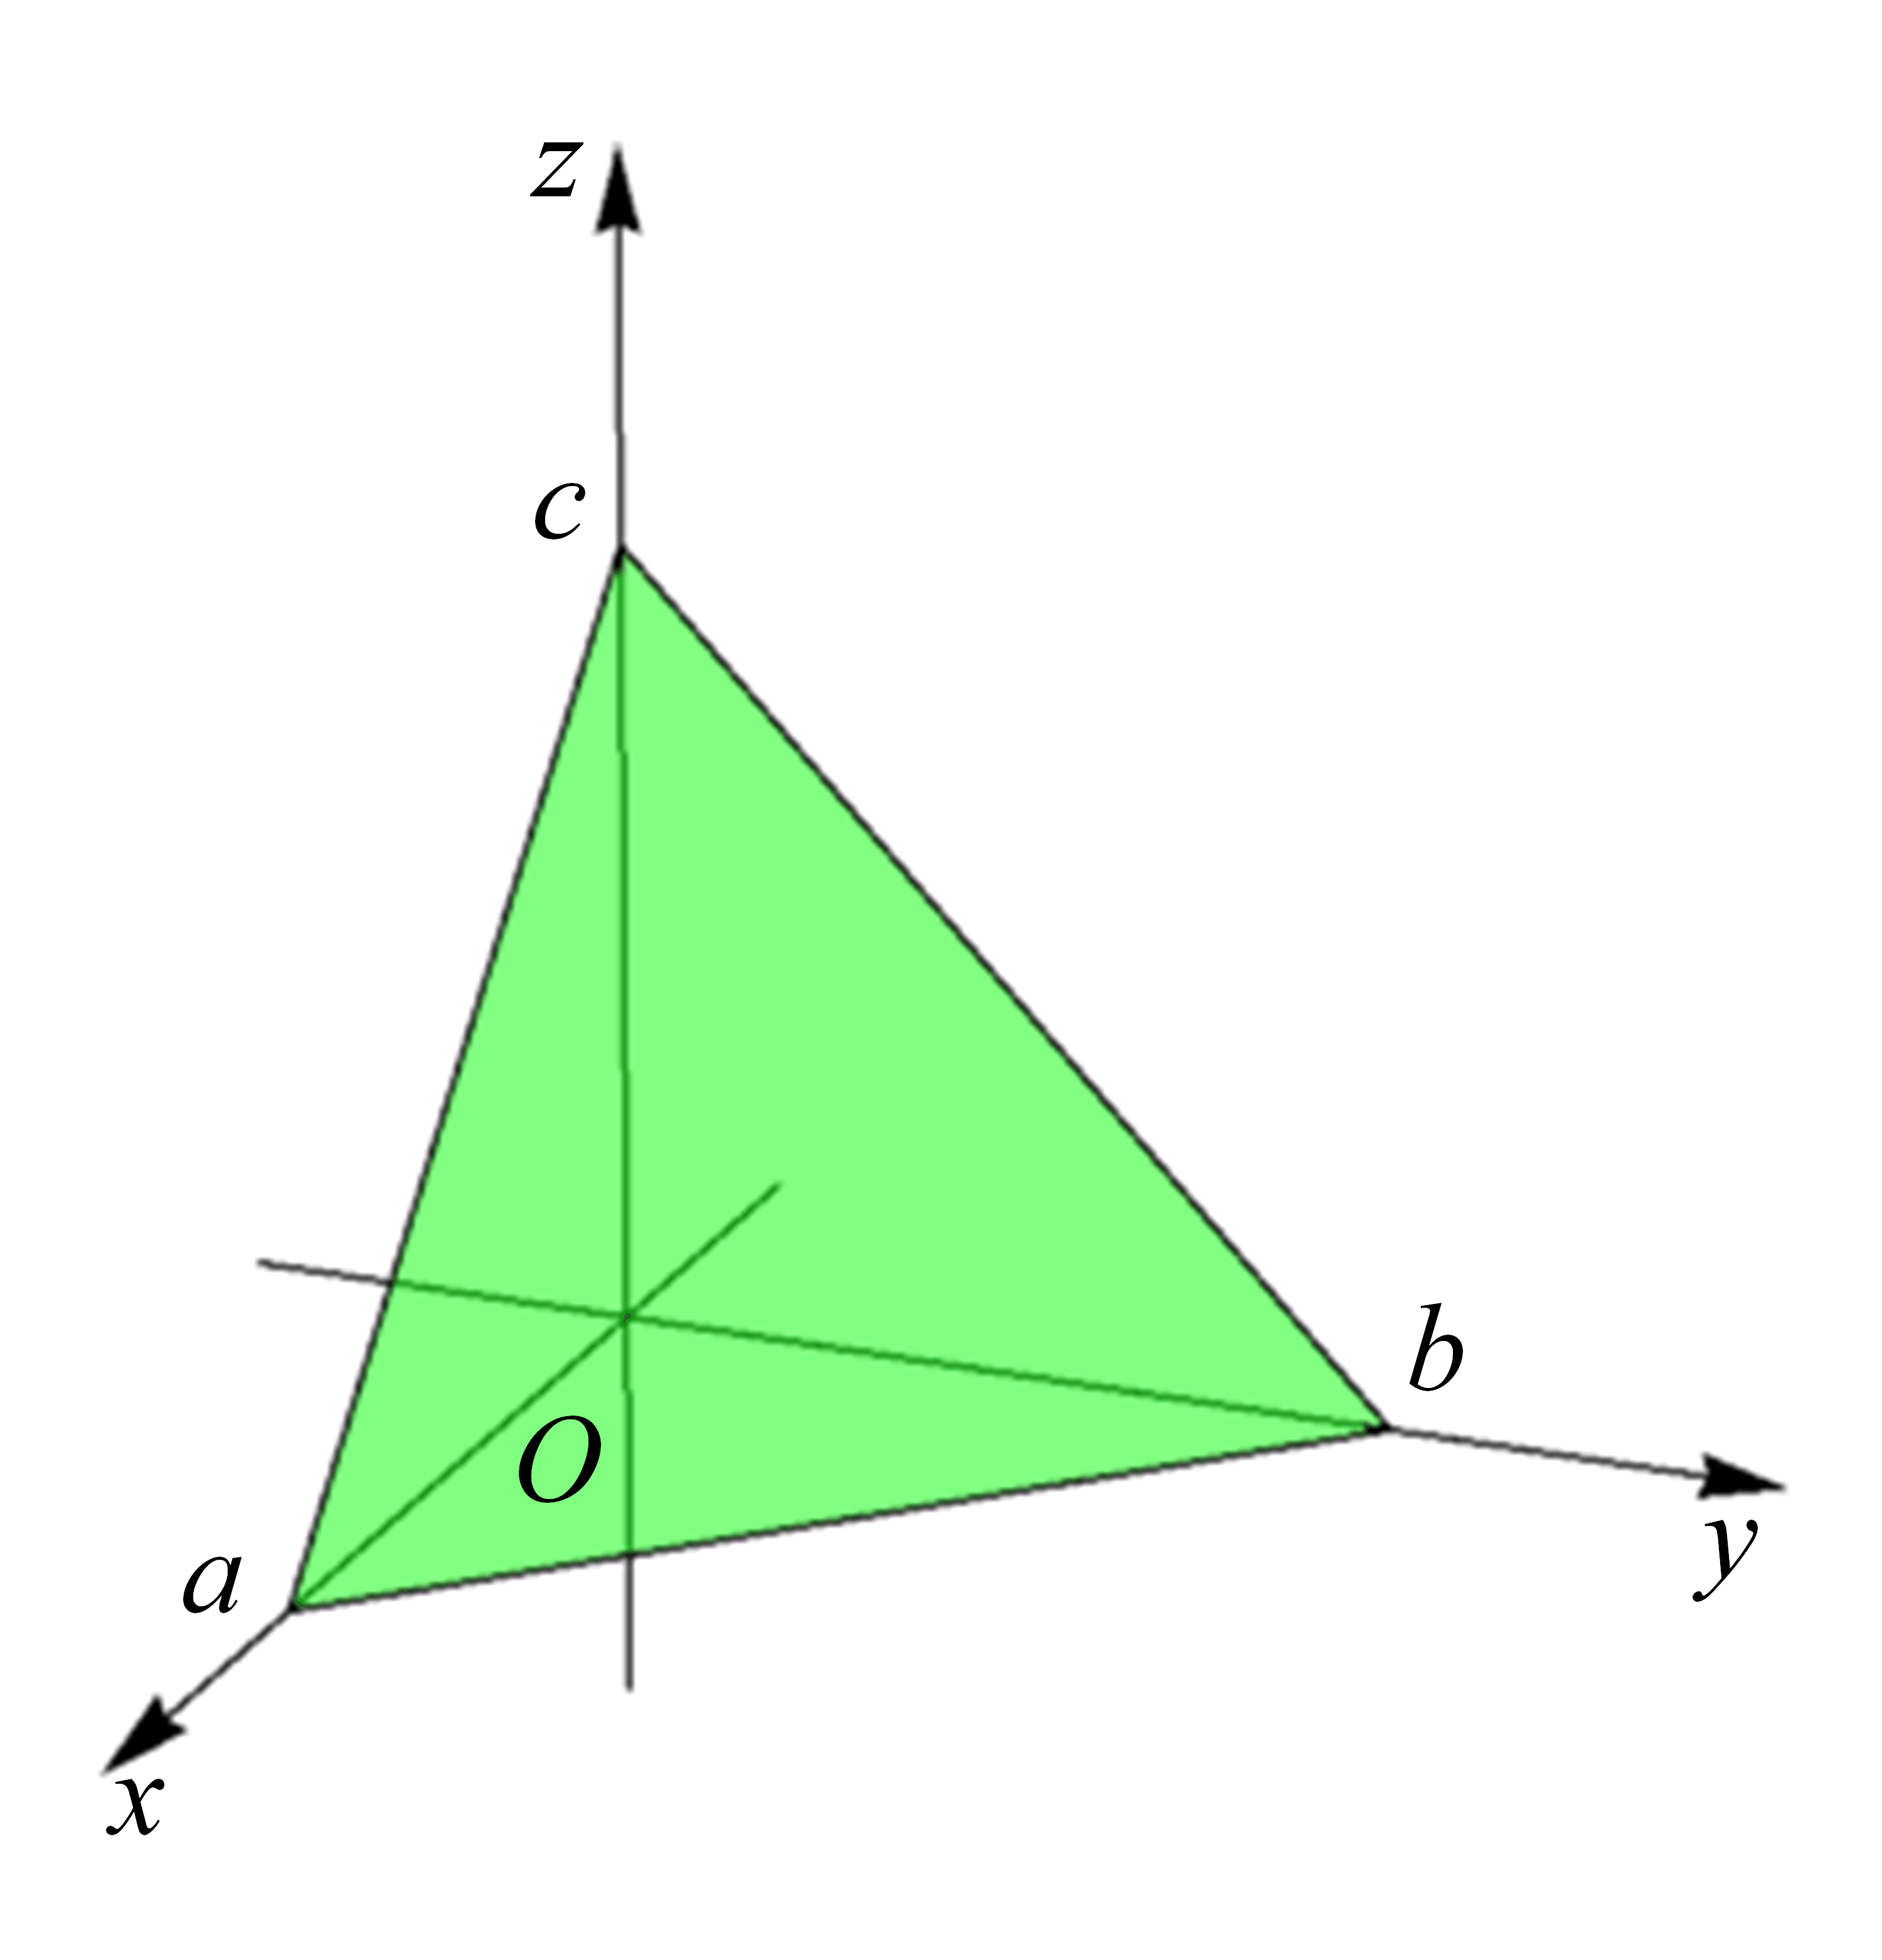
\includegraphics[height=0.2\textheight]{Figures20190605/plane.png} }}
	\subfloat[上半球面$z=\sqrt{R^2-x^2-y^2}$]{{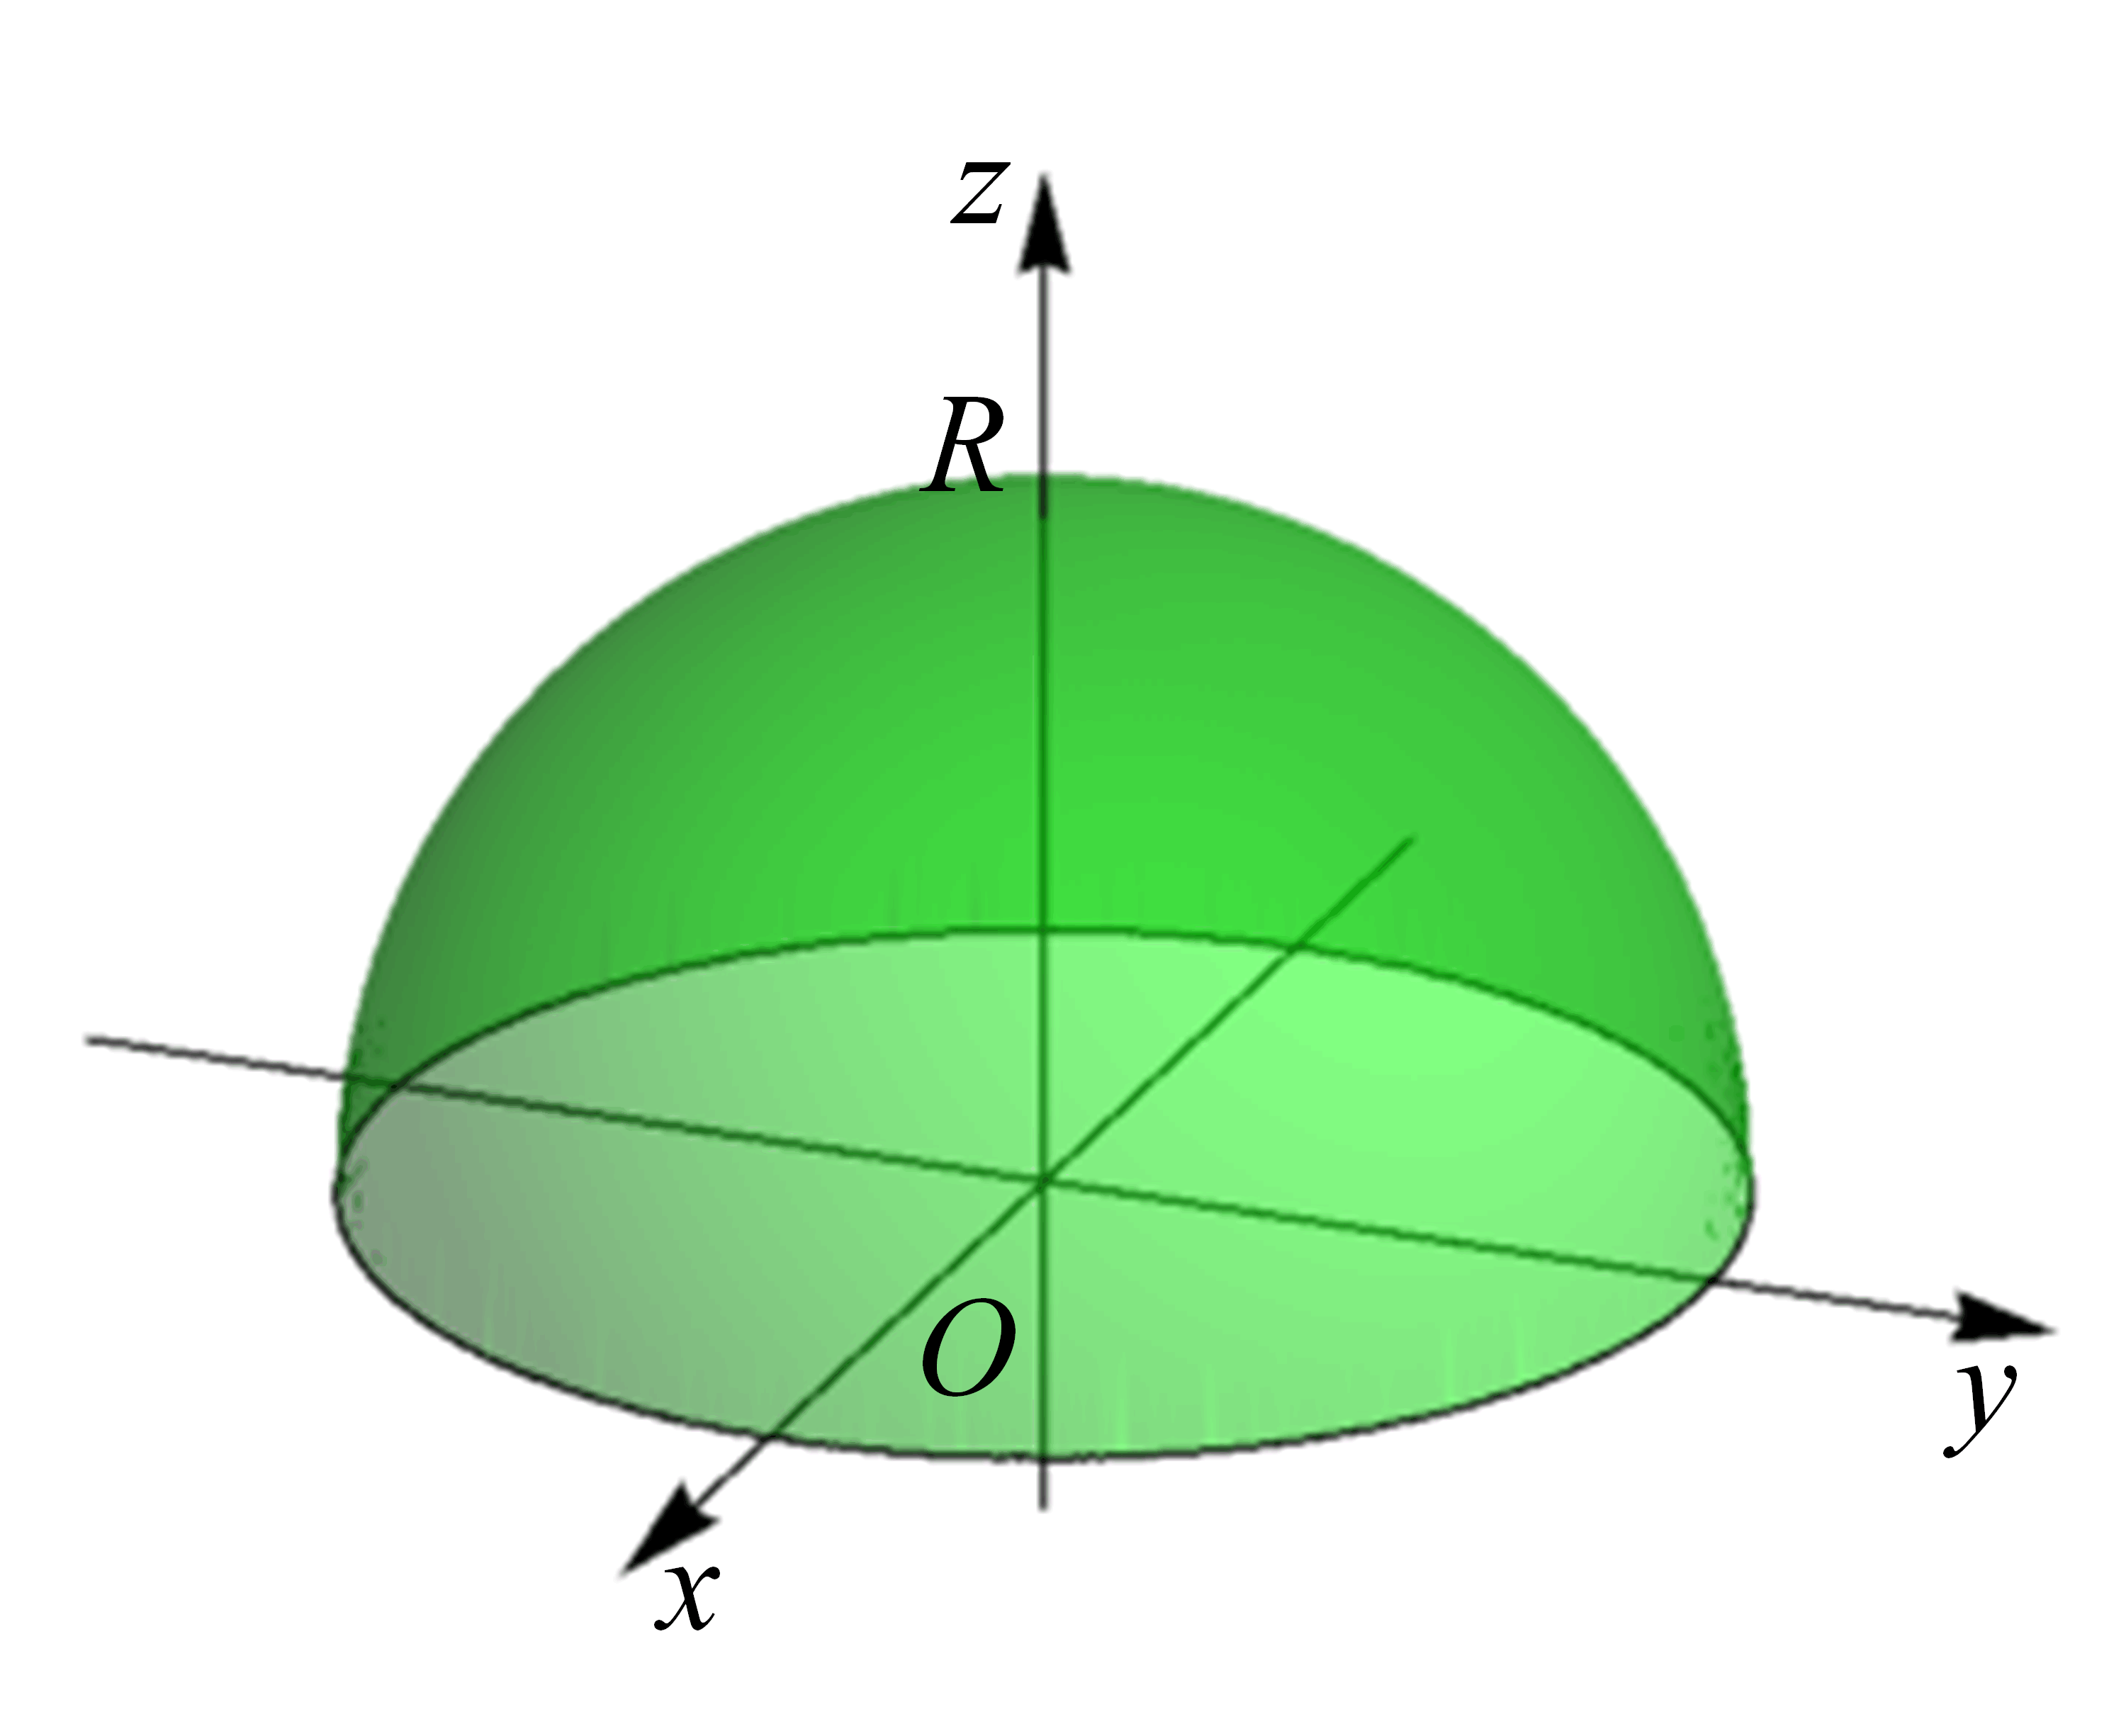
\includegraphics[height=0.2\textheight]{Figures20190605/semisphere.png} }}\\
	\subfloat[上半锥面$z=k\sqrt{x^2+y^2}$]{{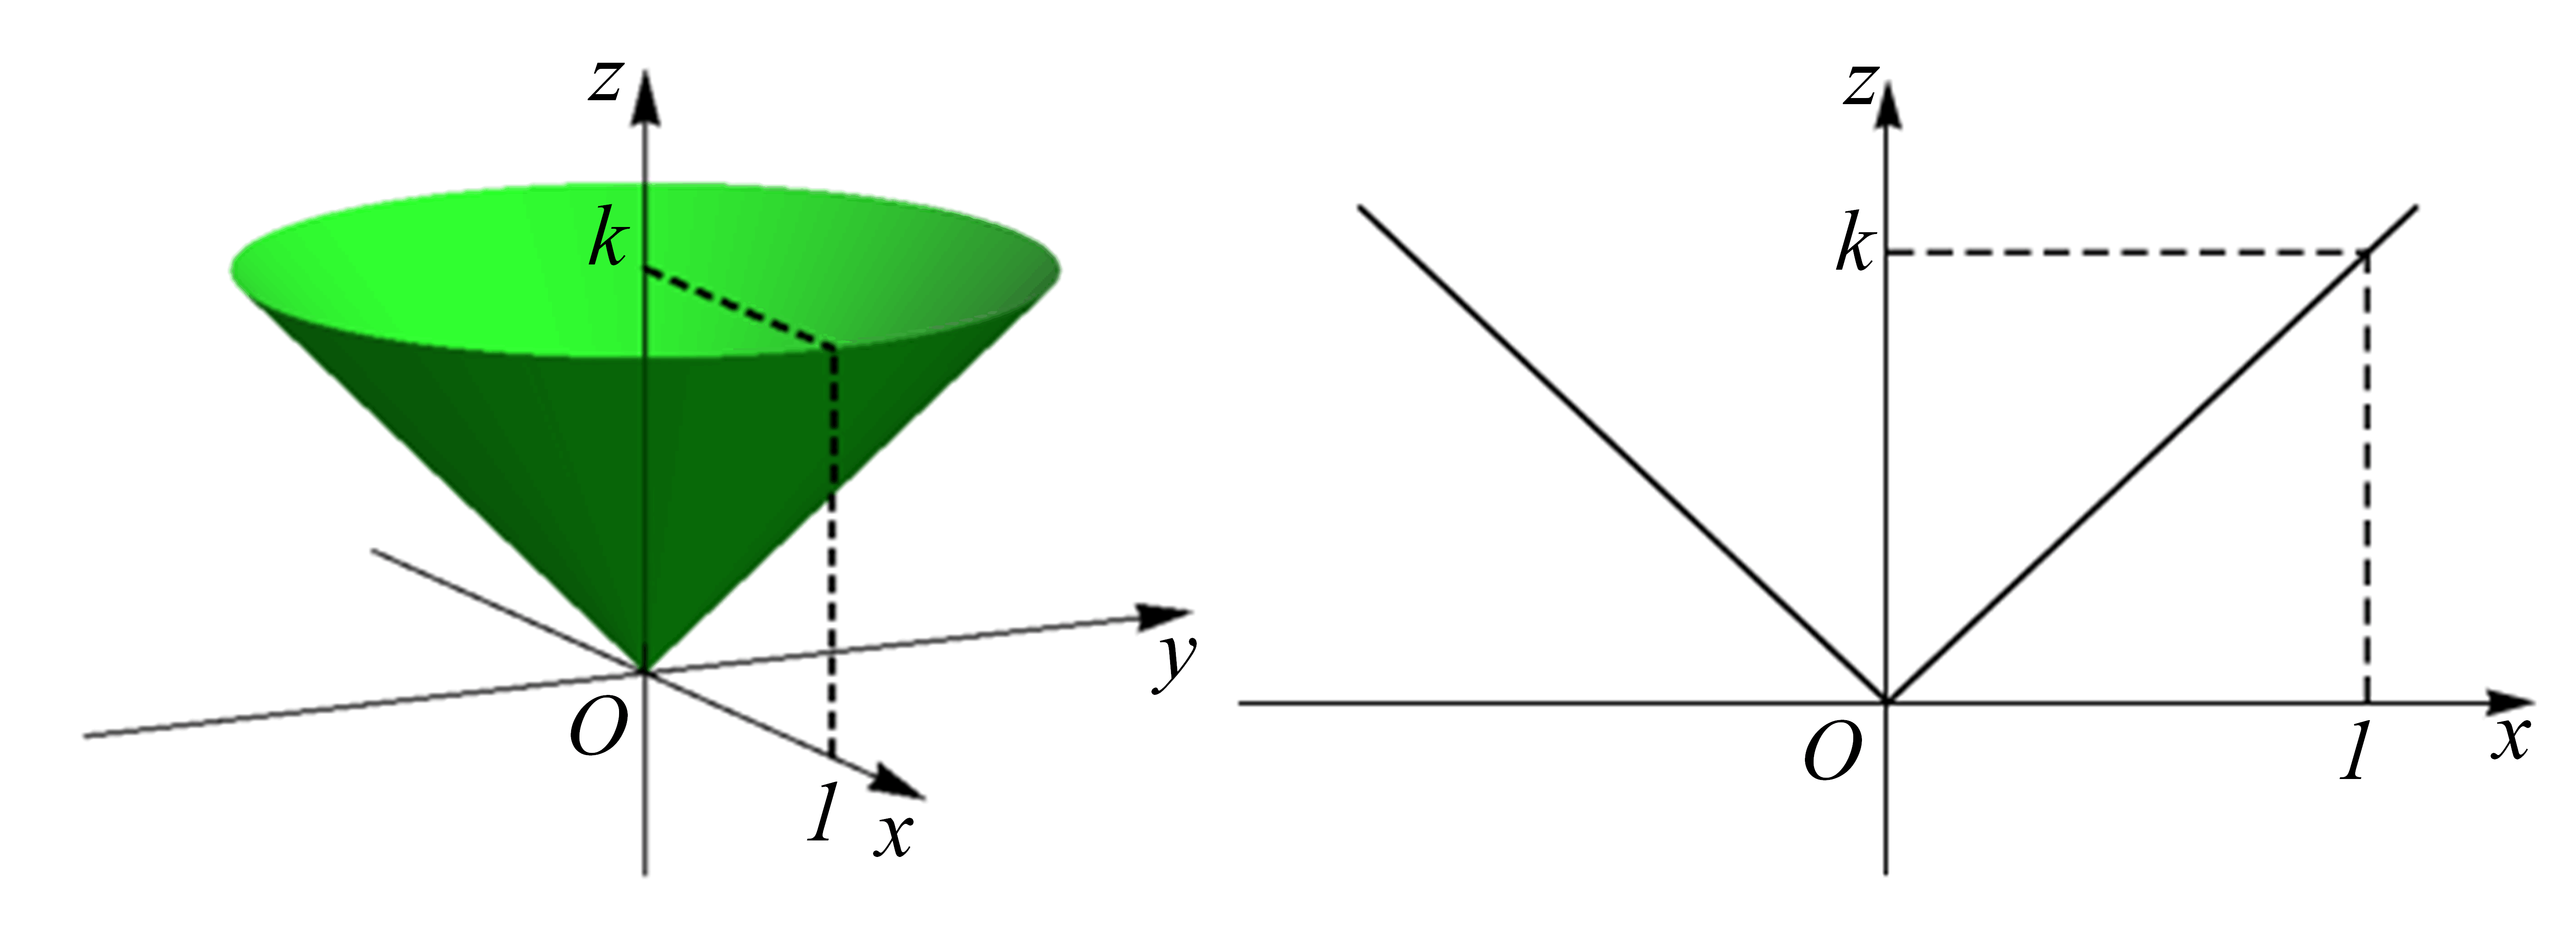
\includegraphics[height=0.16\textheight]{Figures20190605/cone.png} }}\\
	\subfloat[旋转抛物面$z=k(x^2+y^2)$]{{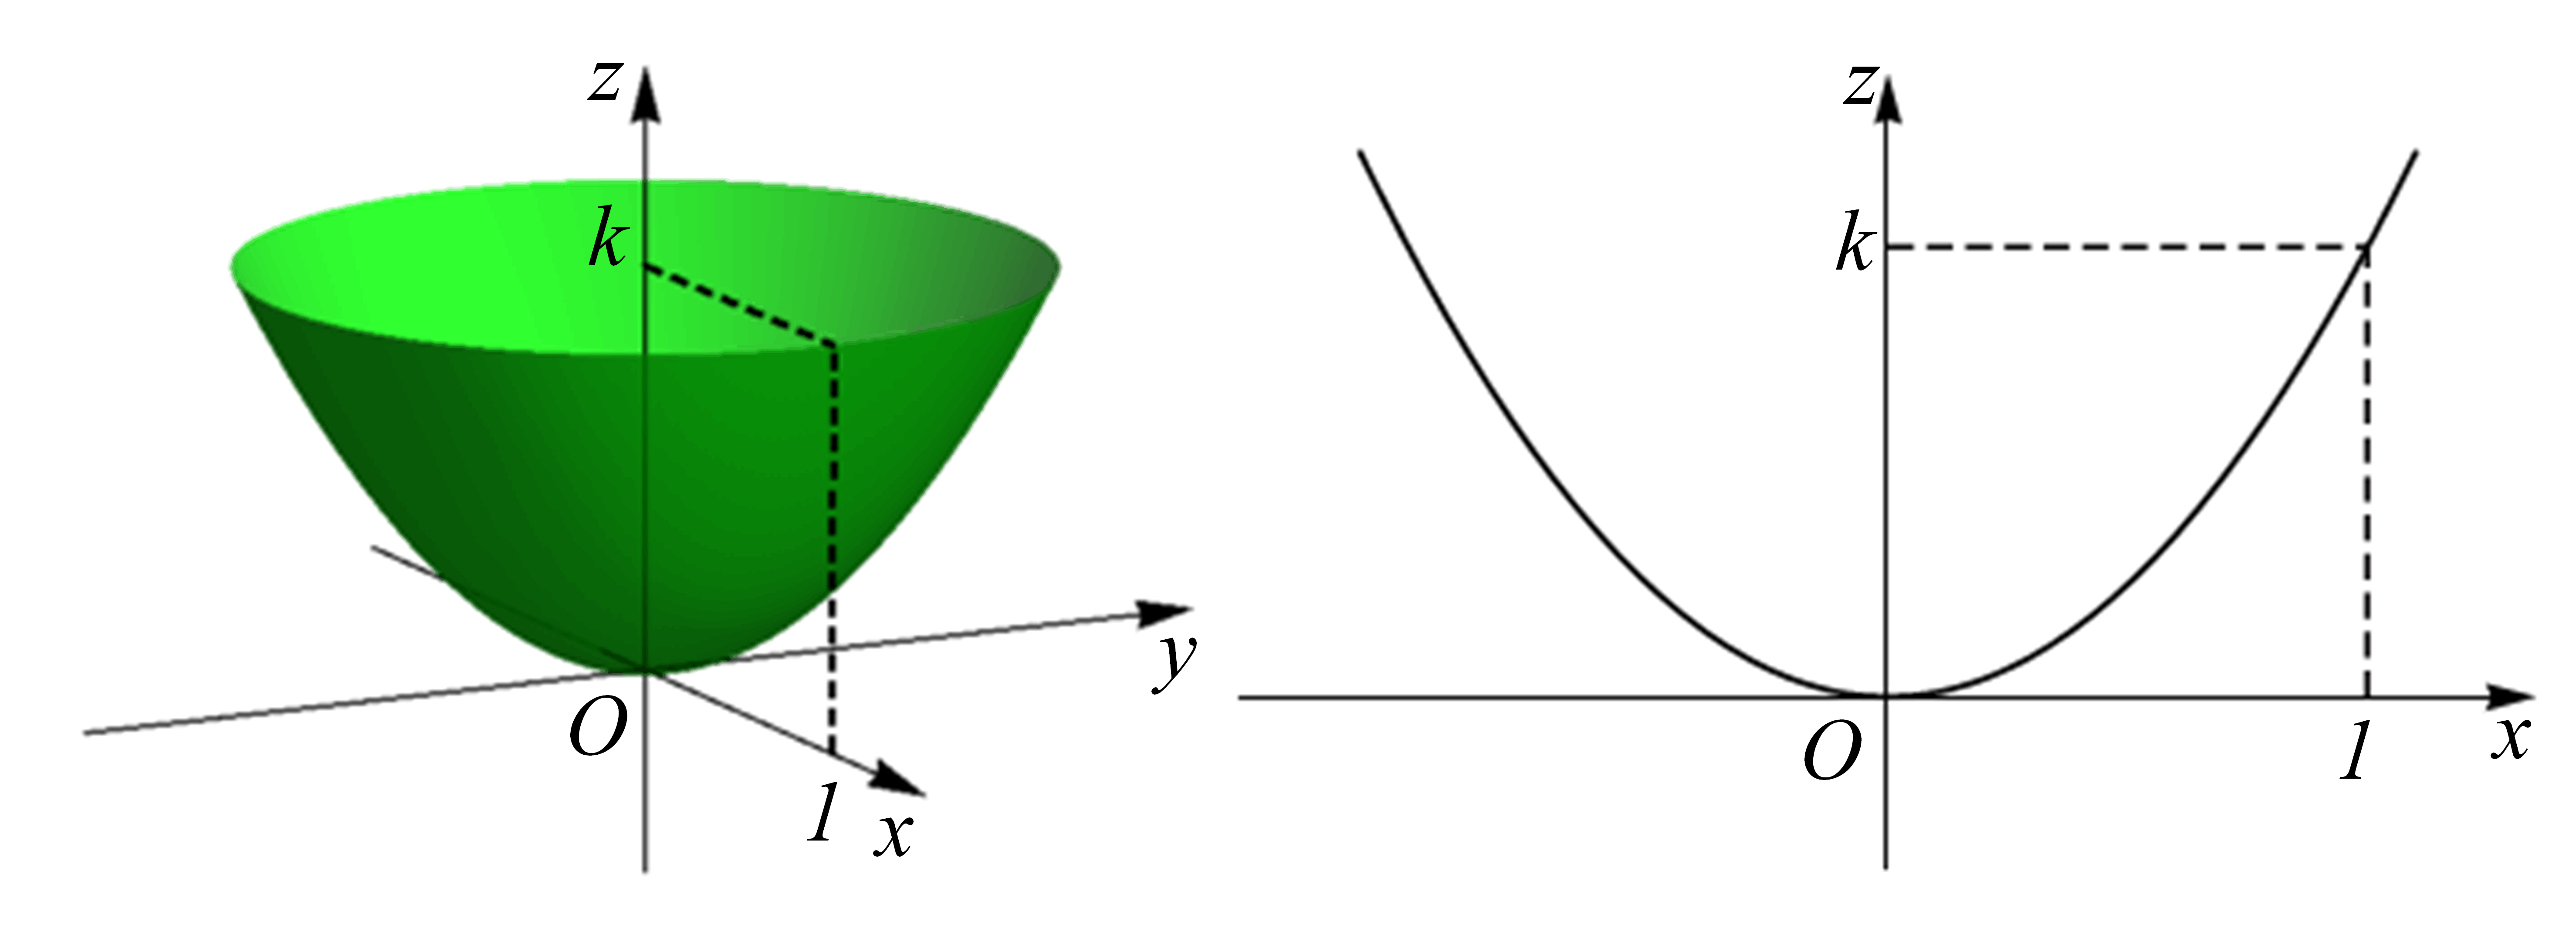
\includegraphics[height=0.16\textheight]{Figures20190605/parabola.png} }}\\
	\subfloat[双曲抛物面(马鞍面)$z=x^2-y^2$和$z=xy$]{{\includegraphics[height=0.2\textheight]{Figures20190605/hyperbola.png} }}
\end{center}
\caption{常见二元函数的图形}
\end{figure}
\item等值线(以双曲抛物面(马鞍面)为例)
\begin{enumerate}
\item[]等值线$\begin{cases}
z=f(x,y),\\
z=c,
\end{cases}$在$xOy$平面上的投影.
\end{enumerate}
\begin{figure}[H]
\begin{center}
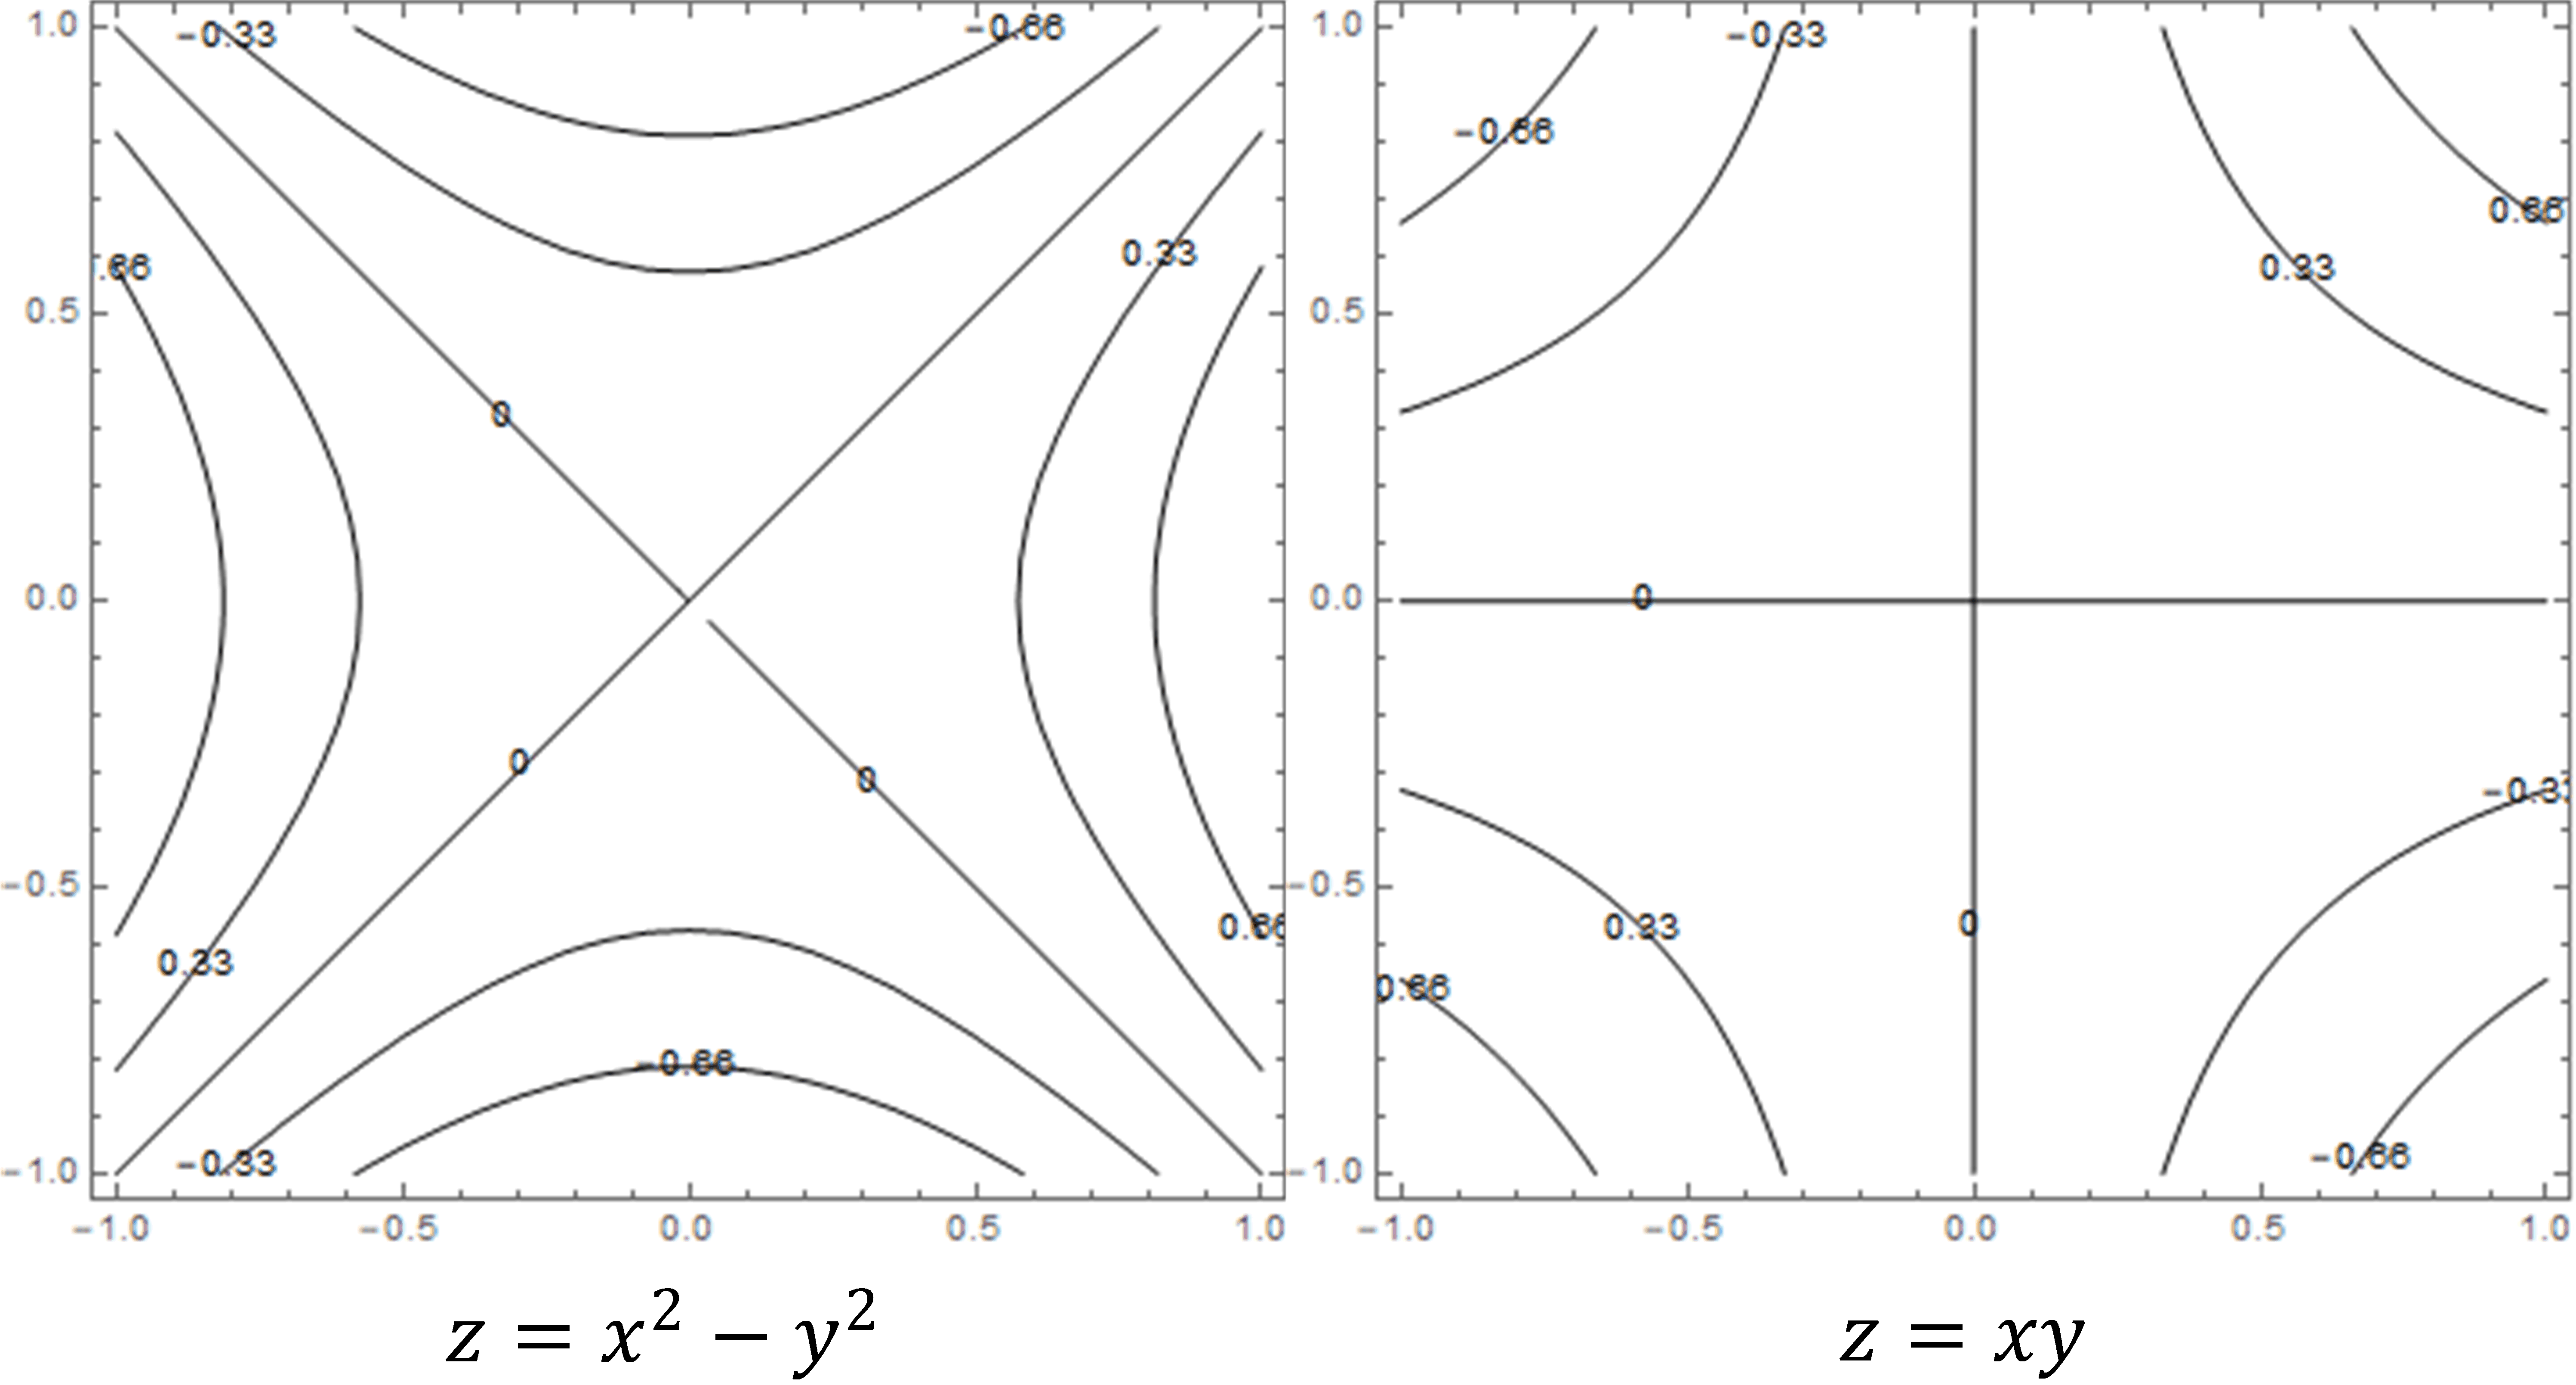
\includegraphics[height=0.3\textheight]{Figures20190605/Contour.png}
\end{center}
\caption{双曲抛物面的等值线}
\end{figure}
\end{enumerate}
\subsection{习题分类与解题思路}
\begin{enumerate}
\item第一类题目:求定义域,主要考虑初等函数对定义域的限制.
\item第二类题目:求极限,解题思路是:
\begin{enumerate}
\item[第1步]尝试构造等价无穷小,或者利用极限的四则运算法则,或者夹逼定理等方法直接求极限。

【如2.(3)/(4)题】
\item[第2步]取特殊路径,看不同路径上的极限是否相等,若不相等则极限不存在,若相等(假设等于$A$)进入第三步;

【如2.(1)题】

\item[第3步]由第二步可知该极限可能等于$A$,利用极限的定义证明函数的极限是或不是$A$. 

\begin{enumerate}
\item[(Yes)]$\forall\varepsilon>0,\exists\delta>0,$当$0<\sqrt{x^2+y^2}<\delta$时$|f(x,y)-A|<\varepsilon$.
\item[(No)]$\exists\varepsilon_0>0,\forall\delta>0$,当$0<\sqrt{x^2+y^2}<\delta$时$|f(x,y)-A|>\varepsilon_0$.
\end{enumerate}

【如2.(2)题】
\end{enumerate}
\item第三类题目:证明连续性. 
\begin{itemize}
\item只需证明函数在其定义域上的任一点处的极限值等于函数值,实质是求极限.

【如3.题】
\item注意三角不等式$d(A,C)-d(B,C)<d(A,B)<d(A,C)+d(B,C)$的使用.
\end{itemize}
\end{enumerate}
\subsection{习题10.1解答}
\begin{enumerate}
\item求下列二元函数的定义域.

\begin{tabular}{ll}
(1)$f(x,y)=\sqrt x\ln(x+y)$;&(2)$f(x,y)=\ln(y-x^2)$;\\
(3)$f(x,y)=\frac{\mathrm e^{\frac xy}}{x-y}$;&(4)$f(x,y)=\arcsin\frac xy$.
\end{tabular}

解:(1)由$x\geq0,x+y>0$得该函数的定义域为$\Set{(x,y)}{x\geq0\text{且}x+y>0}$.

(2)由$y-x^2>0$得该函数的定义域为$\Set{(x,y)}{y>x^2}$.

(3)由$y\neq0$且$x-y^2\neq0$得该函数的定义域为$\Set{(x,y)}{x\neq y^2\text{且}y\neq0}$.

(4)由$y\neq0$且$-1\leq\frac xy\leq1$得该函数的定义域为$\Set{(x,y)}{y\neq0\text{且}-1\leq\frac xy\leq1}$.
\item下列函数在$(0,0)$点的极限是否存在?若存在请求其值.

\begin{tabular}{ll}
(1)$f(x,y)=\frac{x+y}{|x|+|y|}$;&(2)$f(x,y)=\frac{x^2+y^2}{|x|+|y|}$;\\
(3)$f(x,y)=\frac{\sin(x^2+y^2)}{x^2+y^2}$;&(4)$f(x,y)=\frac{1-\cos(xy)}{x^2+y^2}$.
\end{tabular}

解:(1)当点$(x,y)$在第一象限沿直线$y=x$趋于$(0,0)$时$\lim\limits_{\substack{x\rightarrow0^+\\ y\rightarrow0^+}}f(x,y)=\lim\limits_{x\rightarrow0^+}\frac{2x}{2|x|}=1$,

当点$(x,y)$在第二象限沿直线$y=-x$趋于$(0,0)$时$\lim\limits_{\substack{x\rightarrow0^-\\ y\rightarrow0^+}}f(x,y)=\lim\limits_{x\rightarrow0^-}\frac{x-x}{2|x|}=0\neq1$,

故该函数在$(0,0)$点处的极限不存在.

(2)$\because\forall(x,y)\neq(0,0),0<x^2+y^2\leq x^2+y^2+2|x||y|=(|x|+|y|)^2\leq2(x^2+y^2)$

$\therefore\Big|\frac{x^2+y^2}{|x|+|y|}-0\Big|\leq\frac{(|x|+|y|)^2}{|x|+|y|}\leq|x|+|y|\leq\sqrt{2(x^2+y^2)}$

$\therefore\forall\varepsilon>0$可取$\delta=\frac1{\sqrt2}\varepsilon$,当$d((x,y),(0,0))=\sqrt{x^2+y^2}<\delta=\frac1{\sqrt2}\varepsilon$时\\
$\Big|\frac{x^2+y^2}{|x|+|y|}-0\Big|\leq\sqrt{2(x^2+y^2)}<\varepsilon$

$\therefore\lim\limits_{\substack{x\rightarrow0\\ y\rightarrow0}}f(x,y)=0$.

(3)方法1:$\lim\limits_{\substack{x\rightarrow0\\ y\rightarrow0}}f(x,y)=\lim\limits_{\substack{x\rightarrow0\\ y\rightarrow0}}\frac{\sin(x^2+y^2)}{x^2+y^2}=\lim\limits_{\substack{x\rightarrow0\\ y\rightarrow0}}\frac{x^2+y^2}{x^2+y^2}=1$.

方法2:$\because\forall(x,y)\neq(0,0)(\text{不妨设$0<x^2+y^2<\frac\pi2$}),0<\sin(x^2+y^2)<x^2+y^2<\tan(x^2+y^2)$

$\therefore1<\frac{x^2+y^2}{\sin(x^2+y^2)}<\frac1{\cos(x^2+y^2)}$,即$\cos(x^2+y^2)<\frac{\sin(x^2+y^2)}{x^2+y^2}<1$

$\because\lim\limits_{\substack{x\rightarrow0\\ y\rightarrow0}}\cos(x^2+y^2)=1$

$\therefore\lim\limits_{\substack{x\rightarrow0\\ y\rightarrow0}}f(x,y)=1$.

(4)方法1:$\lim\limits_{\substack{x\rightarrow0\\ y\rightarrow0}}f(x,y)=\lim\limits_{\substack{x\rightarrow0\\ y\rightarrow0}}\frac{1-\cos(xy)}{x^2+y^2}=\lim\limits_{\substack{x\rightarrow0\\ y\rightarrow0}}\frac{2\sin^2(\frac{xy}2)}{x^2+y^2}=\lim\limits_{\substack{x\rightarrow0\\ y\rightarrow0}}\frac{2(xy)^2}{4(x^2+y^2)}=\frac12\lim\limits_{\substack{x\rightarrow0\\ y\rightarrow0}}\frac1{\frac1{x^2}+\frac1{y^2}}=0$.

方法2:$\because\Big|\frac{1-\cos(xy)}{x^2+y^2}-0\Big|=\frac{2\sin^2(\frac{xy}2)}{x^2+y^2}\leq\frac{2(\frac{xy}2)^2}{x^2+y^2}\leq\frac{\frac12[\frac12(x^2+y^2)]^2}{x^2+y^2}=\frac18(x^2+y^2)$,

$\therefore\forall\varepsilon>0$取$\delta=\sqrt{8\varepsilon}$,当$0<d((x,y),(0,0))=\sqrt{x^2+y^2}<\delta=\sqrt{8\varepsilon}$时$\Big|\frac{1-\cos(xy)}{x^2+y^2}-0\Big|\\
\leq\frac18(x^2+y^2)<\varepsilon$,

$\therefore\lim\limits_{\substack{x\rightarrow0\\ y\rightarrow0}}f(x,y)=0$.
\item设$P_0$是$\mathbb R^2$中一个确定点,在$\mathbb R^2$上定义函数$f(P)=d(P,P_0)$,求证这是一个连续函数.

证明:方法1:$\because\forall Q\in\mathbb R^2,|d(P,P_0)-d(Q,P_0)|<d(P,Q)$

$\therefore\forall\varepsilon>0$取$\delta=\varepsilon$,当$d(P,Q)<\delta=\varepsilon$时$|d(P,P_0)-d(Q,P_0)|<d(P,Q)<\varepsilon$

$\therefore\lim\limits_{P\rightarrow Q}f(P)=f(Q)$

$\therefore$函数$f(P)$是一个连续函数.

方法2:$\because\forall Q\in\mathbb R^2,d(Q,P_0)-d(Q,P)\leq d(P,P_0)\leq d(Q,P_0)+d(Q,P)$

当$P\rightarrow Q$时$\lim\limits_{P\rightarrow Q}d(Q,P)=0$,根据夹逼定理$\lim\limits_{P\rightarrow Q}d(P,P_0)=d(Q,P_0)$,即$\lim\limits_{P\rightarrow Q}f(P)=f(Q)$

$\therefore$函数$f(P)$是一个连续函数.
\end{enumerate}
\end{document}